\documentclass[twoside]{book}

% Packages required by doxygen
\usepackage{calc}
\usepackage{doxygen}
\usepackage{graphicx}
\usepackage[utf8]{inputenc}
\usepackage{makeidx}
\usepackage{multicol}
\usepackage{multirow}
\usepackage{textcomp}
\usepackage[table]{xcolor}

% Font selection
\usepackage[T1]{fontenc}
\usepackage{mathptmx}
\usepackage[scaled=.90]{helvet}
\usepackage{courier}
\usepackage{amssymb}
\usepackage{sectsty}
\renewcommand{\familydefault}{\sfdefault}
\allsectionsfont{%
  \fontseries{bc}\selectfont%
  \color{darkgray}%
}
\renewcommand{\DoxyLabelFont}{%
  \fontseries{bc}\selectfont%
  \color{darkgray}%
}

% Page & text layout
\usepackage{geometry}
\geometry{%
  a4paper,%
  top=2.5cm,%
  bottom=2.5cm,%
  left=2.5cm,%
  right=2.5cm%
}
\tolerance=750
\hfuzz=15pt
\hbadness=750
\setlength{\emergencystretch}{15pt}
\setlength{\parindent}{0cm}
\setlength{\parskip}{0.2cm}
\makeatletter
\renewcommand{\paragraph}{%
  \@startsection{paragraph}{4}{0ex}{-1.0ex}{1.0ex}{%
    \normalfont\normalsize\bfseries\SS@parafont%
  }%
}
\renewcommand{\subparagraph}{%
  \@startsection{subparagraph}{5}{0ex}{-1.0ex}{1.0ex}{%
    \normalfont\normalsize\bfseries\SS@subparafont%
  }%
}
\makeatother

% Headers & footers
\usepackage{fancyhdr}
\pagestyle{fancyplain}
\fancyhead[LE]{\fancyplain{}{\bfseries\thepage}}
\fancyhead[CE]{\fancyplain{}{}}
\fancyhead[RE]{\fancyplain{}{\bfseries\leftmark}}
\fancyhead[LO]{\fancyplain{}{\bfseries\rightmark}}
\fancyhead[CO]{\fancyplain{}{}}
\fancyhead[RO]{\fancyplain{}{\bfseries\thepage}}
\fancyfoot[LE]{\fancyplain{}{}}
\fancyfoot[CE]{\fancyplain{}{}}
\fancyfoot[RE]{\fancyplain{}{\bfseries\scriptsize Generated on Tue Aug 9 2016 13\-:27\-:37 for Sogo by Doxygen }}
\fancyfoot[LO]{\fancyplain{}{\bfseries\scriptsize Generated on Tue Aug 9 2016 13\-:27\-:37 for Sogo by Doxygen }}
\fancyfoot[CO]{\fancyplain{}{}}
\fancyfoot[RO]{\fancyplain{}{}}
\renewcommand{\footrulewidth}{0.4pt}
\renewcommand{\chaptermark}[1]{%
  \markboth{#1}{}%
}
\renewcommand{\sectionmark}[1]{%
  \markright{\thesection\ #1}%
}

% Indices & bibliography
\usepackage{natbib}
\usepackage[titles]{tocloft}
\setcounter{tocdepth}{3}
\setcounter{secnumdepth}{5}
\makeindex

% Hyperlinks (required, but should be loaded last)
\usepackage{ifpdf}
\ifpdf
  \usepackage[pdftex,pagebackref=true]{hyperref}
\else
  \usepackage[ps2pdf,pagebackref=true]{hyperref}
\fi
\hypersetup{%
  colorlinks=true,%
  linkcolor=blue,%
  citecolor=blue,%
  unicode%
}

% Custom commands
\newcommand{\clearemptydoublepage}{%
  \newpage{\pagestyle{empty}\cleardoublepage}%
}


%===== C O N T E N T S =====

\begin{document}

% Titlepage & ToC
\hypersetup{pageanchor=false}
\pagenumbering{roman}
\begin{titlepage}
\vspace*{7cm}
\begin{center}%
{\Large Sogo \\[1ex]\large 1.\-0 }\\
\vspace*{1cm}
{\large Generated by Doxygen 1.8.6}\\
\vspace*{0.5cm}
{\small Tue Aug 9 2016 13:27:37}\\
\end{center}
\end{titlepage}
\clearemptydoublepage
\tableofcontents
\clearemptydoublepage
\pagenumbering{arabic}
\hypersetup{pageanchor=true}

%--- Begin generated contents ---
\chapter{Sogo Documentation}
\label{index}\hypertarget{index}{}\begin{DoxyAuthor}{Authors}
Nils Brandt 

Alexander Luedke
\end{DoxyAuthor}
\begin{DoxyDate}{Date}
08. August 2016
\end{DoxyDate}
\hypertarget{index_Introduction}{}\section{Introduction}\label{index_Introduction}
This documentation shows the header files of the project sogo wich was develeped\par
 for the education \char`\"{}essensials fo the mobile applications\char`\"{}. 

The complete sourcecode and documentation is located in the \href{https://github.com/alexanderTex/belegEMMS}{\tt repository on Github}. \par
 It can download direct via \par
 git clone \href{https://github.com/alexanderTex/belegEMMS.git}{\tt https\-://github.\-com/alexander\-Tex/beleg\-E\-M\-M\-S.\-git}





\section*{file locations}

\subsubsection*{src/core}


\begin{DoxyItemize}
\item A\-I.\-cpp
\item Gamedata.\-cpp
\item Game\-Manager\-Thread.\-cpp
\item History\-Save.\-cpp
\item Player.\-cpp
\item Play\-Field.\-cpp
\item Vector2.\-cpp
\item Vector3.\-cpp
\end{DoxyItemize}

\subsubsection*{src/gui}


\begin{DoxyItemize}
\item Game\-Input\-Area.\-cpp
\item Game\-View.\-cpp
\item Game\-View2\-D.\-cpp
\item Game\-View3\-D.\-cpp
\item Game\-Visualizer.\-cpp
\item Graphics\-Slot2d.\-cpp
\item Highscore\-Menu.\-cpp
\item History\-Display.\-cpp
\item mainwindow.\-cpp
\item New\-Session\-Menu.\-cpp
\item Pause\-Menu.\-cpp
\item Player\-Input.\-cpp
\item Start\-Menu.\-cpp
\end{DoxyItemize}

\subsubsection*{src/utility}


\begin{DoxyItemize}
\item Logger.\-cpp
\end{DoxyItemize}

\subsubsection*{include/core}


\begin{DoxyItemize}
\item \hyperlink{AI_8h_source}{A\-I.\-h}
\item \hyperlink{GameData_8h_source}{Game\-Data.\-h}
\item \hyperlink{GameManagerThread_8h_source}{Game\-Manager\-Thread.\-h}
\item \hyperlink{HistorySave_8h_source}{History\-Save.\-h}
\item \hyperlink{Player_8h_source}{Player.\-h}
\item \hyperlink{PlayingField_8h_source}{Playing\-Field.\-h}
\item \hyperlink{Vector2_8h_source}{Vector2.\-h}
\item \hyperlink{Vector3_8h_source}{Vector3.\-h}
\end{DoxyItemize}

\subsubsection*{include/gui}


\begin{DoxyItemize}
\item \hyperlink{GameInputArea_8h_source}{Game\-Input\-Area.\-h}
\item \hyperlink{GameView_8h_source}{Game\-View.\-h}
\item \hyperlink{GameView2D_8h_source}{Game\-View2\-D.\-h}
\item \hyperlink{GameView3D_8h_source}{Game\-View3\-D.\-h}
\item \hyperlink{GameVisualizer_8h_source}{Game\-Visualizer.\-h}
\item \hyperlink{GraphicsSlot2d_8h_source}{Graphics\-Slot2d.\-h}
\item \hyperlink{HighscoreMenu_8h_source}{Highscore\-Menu.\-h}
\item \hyperlink{HistoryDisplay_8h_source}{History\-Display.\-h}
\item \hyperlink{mainwindow_8h_source}{mainwindow.\-h}
\item \hyperlink{NewSessionMenu_8h_source}{New\-Session\-Menu.\-h}
\item \hyperlink{PauseMenu_8h_source}{Pause\-Menu.\-h}
\item \hyperlink{PlayerInput_8h_source}{Player\-Input.\-h}
\item \hyperlink{StartMenu_8h_source}{Start\-Menu.\-h}
\end{DoxyItemize}

\subsubsection*{include/utility}


\begin{DoxyItemize}
\item \hyperlink{Logger_8h_source}{Logger.\-h}
\end{DoxyItemize}

\subsubsection*{external}

There are also open\-G\-L files for using the 3\-D component, which is an \char`\"{}merge-\/project\char`\"{} with the education \char`\"{}computer graphic\char`\"{}. \par
 These files are not included in this documentation. 
\chapter{Hierarchical Index}
\section{Class Hierarchy}
This inheritance list is sorted roughly, but not completely, alphabetically\-:\begin{DoxyCompactList}
\item \contentsline{section}{A\-I}{\pageref{classAI}}{}
\item \contentsline{section}{Game\-Manager\-:\-:A\-I\-Player}{\pageref{structGameManager_1_1AIPlayer}}{}
\item \contentsline{section}{Game\-Data}{\pageref{classGameData}}{}
\item \contentsline{section}{History\-Save}{\pageref{classHistorySave}}{}
\item \contentsline{section}{I\-Observer}{\pageref{classIObserver}}{}
\item \contentsline{section}{Logger}{\pageref{classLogger}}{}
\item \contentsline{section}{Player}{\pageref{classPlayer}}{}
\item \contentsline{section}{Playing\-Field}{\pageref{classPlayingField}}{}
\item Q\-Graphics\-Object\begin{DoxyCompactList}
\item \contentsline{section}{Graphics\-Slot2\-D}{\pageref{classGraphicsSlot2D}}{}
\end{DoxyCompactList}
\item Q\-Main\-Window\begin{DoxyCompactList}
\item \contentsline{section}{Main\-Window}{\pageref{classMainWindow}}{}
\end{DoxyCompactList}
\item Q\-Open\-G\-L\-Widget\begin{DoxyCompactList}
\item \contentsline{section}{Game\-View3\-D}{\pageref{classGameView3D}}{}
\end{DoxyCompactList}
\item Q\-Tab\-Widget\begin{DoxyCompactList}
\item \contentsline{section}{Game\-Visualizer}{\pageref{classGameVisualizer}}{}
\end{DoxyCompactList}
\item Q\-Thread\begin{DoxyCompactList}
\item \contentsline{section}{Game\-Manager}{\pageref{classGameManager}}{}
\end{DoxyCompactList}
\item Q\-Widget\begin{DoxyCompactList}
\item \contentsline{section}{Game\-View}{\pageref{classGameView}}{}
\item \contentsline{section}{Game\-View2\-D}{\pageref{classGameView2D}}{}
\item \contentsline{section}{Highscore\-Menu}{\pageref{classHighscoreMenu}}{}
\item \contentsline{section}{History\-Display}{\pageref{classHistoryDisplay}}{}
\item \contentsline{section}{New\-Session\-Menu}{\pageref{classNewSessionMenu}}{}
\item \contentsline{section}{Pause\-Menu}{\pageref{classPauseMenu}}{}
\item \contentsline{section}{Player\-Input}{\pageref{classPlayerInput}}{}
\item \contentsline{section}{Start\-Menu}{\pageref{classStartMenu}}{}
\end{DoxyCompactList}
\item \contentsline{section}{Playing\-Field\-:\-:Slot}{\pageref{structPlayingField_1_1Slot}}{}
\item \contentsline{section}{Subject}{\pageref{classSubject}}{}
\item \contentsline{section}{Vector2}{\pageref{structVector2}}{}
\item \contentsline{section}{Vector3}{\pageref{structVector3}}{}
\end{DoxyCompactList}

\chapter{Class Index}
\section{Class List}
Here are the classes, structs, unions and interfaces with brief descriptions\-:\begin{DoxyCompactList}
\item\contentsline{section}{\hyperlink{classAI}{A\-I} \\*The \hyperlink{classAI}{A\-I} class }{\pageref{classAI}}{}
\item\contentsline{section}{\hyperlink{structGameManager_1_1AIPlayer}{Game\-Manager\-::\-A\-I\-Player} \\*The \hyperlink{classAI}{A\-I} struct Contains a reference to a player which is of type ai and if the ai player has calculated its next move }{\pageref{structGameManager_1_1AIPlayer}}{}
\item\contentsline{section}{\hyperlink{classGameData}{Game\-Data} \\*The \hyperlink{classGameData}{Game\-Data} class Holds a reference to the \hyperlink{classPlayingField}{Playing\-Field} to both players and which one is the currentplayer }{\pageref{classGameData}}{}
\item\contentsline{section}{\hyperlink{classGameManager}{Game\-Manager} \\*The \hyperlink{classGameManager}{Game\-Manager} class Handles the game loop logic in a thread }{\pageref{classGameManager}}{}
\item\contentsline{section}{\hyperlink{classGameView}{Game\-View} \\*The \hyperlink{classGameView}{Game\-View} class }{\pageref{classGameView}}{}
\item\contentsline{section}{\hyperlink{classGameView2D}{Game\-View2\-D} \\*The \hyperlink{classGameView2D}{Game\-View2\-D} class }{\pageref{classGameView2D}}{}
\item\contentsline{section}{\hyperlink{classGameView3D}{Game\-View3\-D} \\*The \hyperlink{classGameView3D}{Game\-View3\-D} class }{\pageref{classGameView3D}}{}
\item\contentsline{section}{\hyperlink{classGameVisualizer}{Game\-Visualizer} \\*The \hyperlink{classGameVisualizer}{Game\-Visualizer} class }{\pageref{classGameVisualizer}}{}
\item\contentsline{section}{\hyperlink{classGraphicsSlot2D}{Graphics\-Slot2\-D} \\*The \hyperlink{classGraphicsSlot2D}{Graphics\-Slot2\-D} class }{\pageref{classGraphicsSlot2D}}{}
\item\contentsline{section}{\hyperlink{classHighscoreMenu}{Highscore\-Menu} \\*The \hyperlink{classHighscoreMenu}{Highscore\-Menu} class }{\pageref{classHighscoreMenu}}{}
\item\contentsline{section}{\hyperlink{classHistoryDisplay}{History\-Display} \\*The \hyperlink{classHistoryDisplay}{History\-Display} class }{\pageref{classHistoryDisplay}}{}
\item\contentsline{section}{\hyperlink{classHistorySave}{History\-Save} \\*The \hyperlink{classHistorySave}{History\-Save} class }{\pageref{classHistorySave}}{}
\item\contentsline{section}{\hyperlink{classIObserver}{I\-Observer} \\*The \hyperlink{classIObserver}{I\-Observer} interface Defines a interface of a Observer which can be Notified Is closely related to the abstract \hyperlink{classSubject}{Subject} class }{\pageref{classIObserver}}{}
\item\contentsline{section}{\hyperlink{classLogger}{Logger} \\*The \hyperlink{classLogger}{Logger} class }{\pageref{classLogger}}{}
\item\contentsline{section}{\hyperlink{classMainWindow}{Main\-Window} \\*The \hyperlink{classMainWindow}{Main\-Window} class }{\pageref{classMainWindow}}{}
\item\contentsline{section}{\hyperlink{classNewSessionMenu}{New\-Session\-Menu} \\*The \hyperlink{classNewSessionMenu}{New\-Session\-Menu} class }{\pageref{classNewSessionMenu}}{}
\item\contentsline{section}{\hyperlink{classPauseMenu}{Pause\-Menu} \\*The \hyperlink{classPauseMenu}{Pause\-Menu} class }{\pageref{classPauseMenu}}{}
\item\contentsline{section}{\hyperlink{classPlayer}{Player} \\*The \hyperlink{classPlayer}{Player} class }{\pageref{classPlayer}}{}
\item\contentsline{section}{\hyperlink{classPlayerInput}{Player\-Input} \\*The \hyperlink{classPlayerInput}{Player\-Input} class }{\pageref{classPlayerInput}}{}
\item\contentsline{section}{\hyperlink{classPlayingField}{Playing\-Field} \\*Defines the Properties of a Playingfield }{\pageref{classPlayingField}}{}
\item\contentsline{section}{\hyperlink{structPlayingField_1_1Slot}{Playing\-Field\-::\-Slot} \\*Defines a Gridspace in a Sogo Playingfield It contains the occupationstate of this position in the grid }{\pageref{structPlayingField_1_1Slot}}{}
\item\contentsline{section}{\hyperlink{classStartMenu}{Start\-Menu} \\*The \hyperlink{classStartMenu}{Start\-Menu} class }{\pageref{classStartMenu}}{}
\item\contentsline{section}{\hyperlink{classSubject}{Subject} \\*The \hyperlink{classSubject}{Subject} class }{\pageref{classSubject}}{}
\item\contentsline{section}{\hyperlink{structVector2}{Vector2} \\*Defines a structures that encapsulates a position in 2\-D space }{\pageref{structVector2}}{}
\item\contentsline{section}{\hyperlink{structVector3}{Vector3} \\*Defines a structures that encapsulates a position in 3\-D space }{\pageref{structVector3}}{}
\end{DoxyCompactList}

\chapter{Class Documentation}
\hypertarget{classAI}{\section{A\-I Class Reference}
\label{classAI}\index{A\-I@{A\-I}}
}


The \hyperlink{classAI}{A\-I} class.  




{\ttfamily \#include $<$A\-I.\-h$>$}



\subsection{Detailed Description}
The \hyperlink{classAI}{A\-I} class. 

Defines an A\-I-\/\-Player Future content strenght etc.

\begin{DoxyAuthor}{Author}
Nils Brandt 

Alexander Luedke
\end{DoxyAuthor}
\begin{DoxyDate}{Date}
08. August 2016
\end{DoxyDate}
\begin{DoxyVersion}{Version}
1.\-0 Add Documentation 
\end{DoxyVersion}

\hypertarget{structGameManager_1_1AIPlayer}{\section{Game\-Manager\-:\-:A\-I\-Player Struct Reference}
\label{structGameManager_1_1AIPlayer}\index{Game\-Manager\-::\-A\-I\-Player@{Game\-Manager\-::\-A\-I\-Player}}
}


The \hyperlink{classAI}{A\-I} struct Contains a reference to a player which is of type ai and if the ai player has calculated its next move.  




{\ttfamily \#include $<$Game\-Manager\-Thread.\-h$>$}

\subsection*{Public Member Functions}
\begin{DoxyCompactItemize}
\item 
\hyperlink{structGameManager_1_1AIPlayer_a9c991a2b7151183f89feefe97e6cfbec}{A\-I\-Player} (const \hyperlink{classPlayer}{Player} $\ast$\hyperlink{structGameManager_1_1AIPlayer_a96450dd315805b21d243f80787a53d6e}{player}, bool \hyperlink{structGameManager_1_1AIPlayer_a0930362037e6d84ec3888eacc8c3c10a}{has\-Move}=false)
\begin{DoxyCompactList}\small\item\em \hyperlink{classAI}{A\-I}. \end{DoxyCompactList}\end{DoxyCompactItemize}
\subsection*{Public Attributes}
\begin{DoxyCompactItemize}
\item 
\hypertarget{structGameManager_1_1AIPlayer_a96450dd315805b21d243f80787a53d6e}{const \hyperlink{classPlayer}{Player} $\ast$ \hyperlink{structGameManager_1_1AIPlayer_a96450dd315805b21d243f80787a53d6e}{player}}\label{structGameManager_1_1AIPlayer_a96450dd315805b21d243f80787a53d6e}

\begin{DoxyCompactList}\small\item\em player \end{DoxyCompactList}\item 
\hypertarget{structGameManager_1_1AIPlayer_a0930362037e6d84ec3888eacc8c3c10a}{bool \hyperlink{structGameManager_1_1AIPlayer_a0930362037e6d84ec3888eacc8c3c10a}{has\-Move}}\label{structGameManager_1_1AIPlayer_a0930362037e6d84ec3888eacc8c3c10a}

\begin{DoxyCompactList}\small\item\em has\-Move \end{DoxyCompactList}\end{DoxyCompactItemize}


\subsection{Detailed Description}
The \hyperlink{classAI}{A\-I} struct Contains a reference to a player which is of type ai and if the ai player has calculated its next move. 

\subsection{Constructor \& Destructor Documentation}
\hypertarget{structGameManager_1_1AIPlayer_a9c991a2b7151183f89feefe97e6cfbec}{\index{Game\-Manager\-::\-A\-I\-Player@{Game\-Manager\-::\-A\-I\-Player}!A\-I\-Player@{A\-I\-Player}}
\index{A\-I\-Player@{A\-I\-Player}!GameManager::AIPlayer@{Game\-Manager\-::\-A\-I\-Player}}
\subsubsection[{A\-I\-Player}]{\setlength{\rightskip}{0pt plus 5cm}Game\-Manager\-::\-A\-I\-Player\-::\-A\-I\-Player (
\begin{DoxyParamCaption}
\item[{const {\bf Player} $\ast$}]{player, }
\item[{bool}]{has\-Move = {\ttfamily false}}
\end{DoxyParamCaption}
)\hspace{0.3cm}{\ttfamily [inline]}}}\label{structGameManager_1_1AIPlayer_a9c991a2b7151183f89feefe97e6cfbec}


\hyperlink{classAI}{A\-I}. 


\begin{DoxyParams}{Parameters}
{\em player} & \\
\hline
{\em has\-Move} & \\
\hline
\end{DoxyParams}

\hypertarget{classGameData}{\section{Game\-Data Class Reference}
\label{classGameData}\index{Game\-Data@{Game\-Data}}
}


The \hyperlink{classGameData}{Game\-Data} class Holds a reference to the \hyperlink{classPlayingField}{Playing\-Field} to both players and which one is the currentplayer.  




{\ttfamily \#include $<$Game\-Data.\-h$>$}

\subsection*{Public Types}
\begin{DoxyCompactItemize}
\item 
enum \hyperlink{classGameData_a2cbc881e9ac218f14694fed595c3c128}{Game\-Data\-Exception} \{ {\bfseries Player\-Not\-In\-The\-Game}
 \}
\begin{DoxyCompactList}\small\item\em The Game\-Data\-Exception enum thrown Player\-Not\-In\-The\-Game when the player is not a player of the game. \end{DoxyCompactList}\end{DoxyCompactItemize}
\subsection*{Public Member Functions}
\begin{DoxyCompactItemize}
\item 
\hypertarget{classGameData_a67ab18c5a35df618e99983275c7552ab}{\hyperlink{classGameData_a67ab18c5a35df618e99983275c7552ab}{Game\-Data} ()}\label{classGameData_a67ab18c5a35df618e99983275c7552ab}

\begin{DoxyCompactList}\small\item\em \hyperlink{classGameData}{Game\-Data} Default Constructor. \end{DoxyCompactList}\item 
\hyperlink{classGameData_aea94874f6fb34c81daf86ab294a3e094}{Game\-Data} (\hyperlink{classPlayingField}{Playing\-Field} $\ast$field, \hyperlink{classPlayer}{Player} $\ast$p1, \hyperlink{classPlayer}{Player} $\ast$p2, \hyperlink{classPlayer}{Player} $\ast$starting\-Player)
\begin{DoxyCompactList}\small\item\em \hyperlink{classGameData}{Game\-Data} Initializes a Gamedata object with a given \hyperlink{classPlayingField}{Playing\-Field} both players and the designated starting player. \end{DoxyCompactList}\item 
\hyperlink{classGameData_ae0f631bbb4bf25dd4e3888a5ef9a4eb6}{Game\-Data} (const \hyperlink{classGameData}{Game\-Data} \&src)
\begin{DoxyCompactList}\small\item\em \hyperlink{classGameData}{Game\-Data} Copy Constructor. \end{DoxyCompactList}\item 
\hypertarget{classGameData_abd51e710bc262e278a8895f2e0b35a9f}{virtual \hyperlink{classGameData_abd51e710bc262e278a8895f2e0b35a9f}{$\sim$\-Game\-Data} ()}\label{classGameData_abd51e710bc262e278a8895f2e0b35a9f}

\begin{DoxyCompactList}\small\item\em $\sim$\-Game\-Data \end{DoxyCompactList}\item 
const \hyperlink{classPlayingField}{Playing\-Field} $\ast$ \hyperlink{classGameData_af932f66030087c333f2d5746f9fd555c}{Get\-Field} () const 
\begin{DoxyCompactList}\small\item\em Get\-Field. \end{DoxyCompactList}\item 
std\-::vector$<$ const \hyperlink{classPlayer}{Player} $\ast$ $>$ $\ast$ \hyperlink{classGameData_a423674f3ce9e6283b7262a9187ee0449}{Get\-Players} () const 
\begin{DoxyCompactList}\small\item\em Get\-Players. \end{DoxyCompactList}\item 
\hyperlink{classPlayer}{Player} $\ast$ \hyperlink{classGameData_a1642c300ee35687a67b807cedee9e55d}{Get\-Player1} () const 
\begin{DoxyCompactList}\small\item\em Get\-Player1. \end{DoxyCompactList}\item 
\hyperlink{classPlayer}{Player} $\ast$ \hyperlink{classGameData_aa9012da90297a55f563a20f0b927b051}{Get\-Player2} () const 
\begin{DoxyCompactList}\small\item\em Get\-Player2. \end{DoxyCompactList}\item 
\hyperlink{classPlayer}{Player} $\ast$ \hyperlink{classGameData_a5e07bca98788c169c82e0e0f393755a7}{Get\-Current\-Player} () const 
\begin{DoxyCompactList}\small\item\em Get\-Current\-Player. \end{DoxyCompactList}\item 
\hyperlink{structVector3}{Vector3} \hyperlink{classGameData_a5c754d78e1521b2b32b53a083d5cf7f5}{Get\-Last\-Move} () const 
\begin{DoxyCompactList}\small\item\em Get\-Last\-Move. \end{DoxyCompactList}\item 
const \hyperlink{classPlayer}{Player} $\ast$ \hyperlink{classGameData_a7cf443182a19f49bac785f7224d57d81}{Get\-Opponent} (const \hyperlink{classPlayer}{Player} $\ast$p) const   throw (\-Game\-Data\-Exception)
\begin{DoxyCompactList}\small\item\em Get\-Opponent. \end{DoxyCompactList}\item 
const \hyperlink{classHistorySave}{History\-Save} $\ast$ \hyperlink{classGameData_ad0e34ba7f1106ff9b5fdd8e99f327ec1}{Get\-History} () const 
\begin{DoxyCompactList}\small\item\em Get\-History. \end{DoxyCompactList}\item 
void \hyperlink{classGameData_a5e1d9b00d89fea74a17e653057b47541}{Occupy\-Slot} (int x, int y, int z, \hyperlink{classPlayingField_ac6df152a3f820aa04a00ab4df4a9d265}{Playing\-Field\-::\-Occupation\-State} player\-Color)  throw (out\-\_\-of\-\_\-range, Playing\-Field\-::\-Field\-Exeptions)
\begin{DoxyCompactList}\small\item\em Occupy\-Slot occupies slotint playingfield and adds the move to the move history. \end{DoxyCompactList}\item 
\hypertarget{classGameData_a18924e62415d38e1651ef1ab7d488996}{void \hyperlink{classGameData_a18924e62415d38e1651ef1ab7d488996}{Switch\-Player} ()}\label{classGameData_a18924e62415d38e1651ef1ab7d488996}

\begin{DoxyCompactList}\small\item\em Switch\-Player switch currentplayer to other player. \end{DoxyCompactList}\end{DoxyCompactItemize}
\subsection*{Static Public Member Functions}
\begin{DoxyCompactItemize}
\item 
\hypertarget{classGameData_a5f923199f27169c1c3aa0e4276153fc5}{static string {\bfseries Serialize} (const \hyperlink{classGameData}{Game\-Data} \&data)}\label{classGameData_a5f923199f27169c1c3aa0e4276153fc5}

\item 
\hypertarget{classGameData_a11cecb1c8a834e0928ec5f554d7e9d89}{static \hyperlink{classGameData}{Game\-Data} $\ast$ {\bfseries Deserialize} (std\-::string str)  throw (\-Deserialization\-Exception)}\label{classGameData_a11cecb1c8a834e0928ec5f554d7e9d89}

\end{DoxyCompactItemize}


\subsection{Detailed Description}
The \hyperlink{classGameData}{Game\-Data} class Holds a reference to the \hyperlink{classPlayingField}{Playing\-Field} to both players and which one is the currentplayer. 

\begin{DoxyAuthor}{Author}
Nils Brandt 

Alexander Luedke
\end{DoxyAuthor}
\begin{DoxyDate}{Date}
08. August 2016
\end{DoxyDate}
\begin{DoxyVersion}{Version}
1.\-0 Add Documentation 
\end{DoxyVersion}


\subsection{Constructor \& Destructor Documentation}
\hypertarget{classGameData_aea94874f6fb34c81daf86ab294a3e094}{\index{Game\-Data@{Game\-Data}!Game\-Data@{Game\-Data}}
\index{Game\-Data@{Game\-Data}!GameData@{Game\-Data}}
\subsubsection[{Game\-Data}]{\setlength{\rightskip}{0pt plus 5cm}Game\-Data\-::\-Game\-Data (
\begin{DoxyParamCaption}
\item[{{\bf Playing\-Field} $\ast$}]{field, }
\item[{{\bf Player} $\ast$}]{p1, }
\item[{{\bf Player} $\ast$}]{p2, }
\item[{{\bf Player} $\ast$}]{starting\-Player}
\end{DoxyParamCaption}
)}}\label{classGameData_aea94874f6fb34c81daf86ab294a3e094}


\hyperlink{classGameData}{Game\-Data} Initializes a Gamedata object with a given \hyperlink{classPlayingField}{Playing\-Field} both players and the designated starting player. 


\begin{DoxyParams}{Parameters}
{\em field} & given \hyperlink{classPlayingField}{Playing\-Field} \\
\hline
{\em p1} & player1 \\
\hline
{\em p2} & player2 \\
\hline
{\em starting\-Player} & the beginning player \\
\hline
\end{DoxyParams}
\hypertarget{classGameData_ae0f631bbb4bf25dd4e3888a5ef9a4eb6}{\index{Game\-Data@{Game\-Data}!Game\-Data@{Game\-Data}}
\index{Game\-Data@{Game\-Data}!GameData@{Game\-Data}}
\subsubsection[{Game\-Data}]{\setlength{\rightskip}{0pt plus 5cm}Game\-Data\-::\-Game\-Data (
\begin{DoxyParamCaption}
\item[{const {\bf Game\-Data} \&}]{src}
\end{DoxyParamCaption}
)}}\label{classGameData_ae0f631bbb4bf25dd4e3888a5ef9a4eb6}


\hyperlink{classGameData}{Game\-Data} Copy Constructor. 


\begin{DoxyParams}{Parameters}
{\em src} & Gamedata to copy from \\
\hline
\end{DoxyParams}


\subsection{Member Function Documentation}
\hypertarget{classGameData_a5e07bca98788c169c82e0e0f393755a7}{\index{Game\-Data@{Game\-Data}!Get\-Current\-Player@{Get\-Current\-Player}}
\index{Get\-Current\-Player@{Get\-Current\-Player}!GameData@{Game\-Data}}
\subsubsection[{Get\-Current\-Player}]{\setlength{\rightskip}{0pt plus 5cm}{\bf Player} $\ast$ Game\-Data\-::\-Get\-Current\-Player (
\begin{DoxyParamCaption}
{}
\end{DoxyParamCaption}
) const}}\label{classGameData_a5e07bca98788c169c82e0e0f393755a7}


Get\-Current\-Player. 

\begin{DoxyReturn}{Returns}

\end{DoxyReturn}
\hypertarget{classGameData_af932f66030087c333f2d5746f9fd555c}{\index{Game\-Data@{Game\-Data}!Get\-Field@{Get\-Field}}
\index{Get\-Field@{Get\-Field}!GameData@{Game\-Data}}
\subsubsection[{Get\-Field}]{\setlength{\rightskip}{0pt plus 5cm}const {\bf Playing\-Field} $\ast$ Game\-Data\-::\-Get\-Field (
\begin{DoxyParamCaption}
{}
\end{DoxyParamCaption}
) const}}\label{classGameData_af932f66030087c333f2d5746f9fd555c}


Get\-Field. 

\begin{DoxyReturn}{Returns}

\end{DoxyReturn}
\hypertarget{classGameData_ad0e34ba7f1106ff9b5fdd8e99f327ec1}{\index{Game\-Data@{Game\-Data}!Get\-History@{Get\-History}}
\index{Get\-History@{Get\-History}!GameData@{Game\-Data}}
\subsubsection[{Get\-History}]{\setlength{\rightskip}{0pt plus 5cm}const {\bf History\-Save} $\ast$ Game\-Data\-::\-Get\-History (
\begin{DoxyParamCaption}
{}
\end{DoxyParamCaption}
) const}}\label{classGameData_ad0e34ba7f1106ff9b5fdd8e99f327ec1}


Get\-History. 

\begin{DoxyReturn}{Returns}

\end{DoxyReturn}
\hypertarget{classGameData_a5c754d78e1521b2b32b53a083d5cf7f5}{\index{Game\-Data@{Game\-Data}!Get\-Last\-Move@{Get\-Last\-Move}}
\index{Get\-Last\-Move@{Get\-Last\-Move}!GameData@{Game\-Data}}
\subsubsection[{Get\-Last\-Move}]{\setlength{\rightskip}{0pt plus 5cm}{\bf Vector3} Game\-Data\-::\-Get\-Last\-Move (
\begin{DoxyParamCaption}
{}
\end{DoxyParamCaption}
) const}}\label{classGameData_a5c754d78e1521b2b32b53a083d5cf7f5}


Get\-Last\-Move. 

\begin{DoxyReturn}{Returns}

\end{DoxyReturn}
\hypertarget{classGameData_a7cf443182a19f49bac785f7224d57d81}{\index{Game\-Data@{Game\-Data}!Get\-Opponent@{Get\-Opponent}}
\index{Get\-Opponent@{Get\-Opponent}!GameData@{Game\-Data}}
\subsubsection[{Get\-Opponent}]{\setlength{\rightskip}{0pt plus 5cm}const {\bf Player} $\ast$ Game\-Data\-::\-Get\-Opponent (
\begin{DoxyParamCaption}
\item[{const {\bf Player} $\ast$}]{p}
\end{DoxyParamCaption}
) const throw  {\bf Game\-Data\-Exception}) }}\label{classGameData_a7cf443182a19f49bac785f7224d57d81}


Get\-Opponent. 


\begin{DoxyParams}{Parameters}
{\em p} & \\
\hline
\end{DoxyParams}
\begin{DoxyReturn}{Returns}
throws Gamedata\-Exception if the given player p is not part of the game 
\end{DoxyReturn}
\hypertarget{classGameData_a1642c300ee35687a67b807cedee9e55d}{\index{Game\-Data@{Game\-Data}!Get\-Player1@{Get\-Player1}}
\index{Get\-Player1@{Get\-Player1}!GameData@{Game\-Data}}
\subsubsection[{Get\-Player1}]{\setlength{\rightskip}{0pt plus 5cm}{\bf Player} $\ast$ Game\-Data\-::\-Get\-Player1 (
\begin{DoxyParamCaption}
{}
\end{DoxyParamCaption}
) const}}\label{classGameData_a1642c300ee35687a67b807cedee9e55d}


Get\-Player1. 

\begin{DoxyReturn}{Returns}

\end{DoxyReturn}
\hypertarget{classGameData_aa9012da90297a55f563a20f0b927b051}{\index{Game\-Data@{Game\-Data}!Get\-Player2@{Get\-Player2}}
\index{Get\-Player2@{Get\-Player2}!GameData@{Game\-Data}}
\subsubsection[{Get\-Player2}]{\setlength{\rightskip}{0pt plus 5cm}{\bf Player} $\ast$ Game\-Data\-::\-Get\-Player2 (
\begin{DoxyParamCaption}
{}
\end{DoxyParamCaption}
) const}}\label{classGameData_aa9012da90297a55f563a20f0b927b051}


Get\-Player2. 

\begin{DoxyReturn}{Returns}

\end{DoxyReturn}
\hypertarget{classGameData_a423674f3ce9e6283b7262a9187ee0449}{\index{Game\-Data@{Game\-Data}!Get\-Players@{Get\-Players}}
\index{Get\-Players@{Get\-Players}!GameData@{Game\-Data}}
\subsubsection[{Get\-Players}]{\setlength{\rightskip}{0pt plus 5cm}std\-::vector$<$ const {\bf Player} $\ast$ $>$ $\ast$ Game\-Data\-::\-Get\-Players (
\begin{DoxyParamCaption}
{}
\end{DoxyParamCaption}
) const}}\label{classGameData_a423674f3ce9e6283b7262a9187ee0449}


Get\-Players. 

\begin{DoxyReturn}{Returns}

\end{DoxyReturn}
\hypertarget{classGameData_a5e1d9b00d89fea74a17e653057b47541}{\index{Game\-Data@{Game\-Data}!Occupy\-Slot@{Occupy\-Slot}}
\index{Occupy\-Slot@{Occupy\-Slot}!GameData@{Game\-Data}}
\subsubsection[{Occupy\-Slot}]{\setlength{\rightskip}{0pt plus 5cm}void Game\-Data\-::\-Occupy\-Slot (
\begin{DoxyParamCaption}
\item[{int}]{x, }
\item[{int}]{y, }
\item[{int}]{z, }
\item[{{\bf Playing\-Field\-::\-Occupation\-State}}]{player\-Color}
\end{DoxyParamCaption}
) throw  out\-\_\-of\-\_\-range, {\bf Playing\-Field\-::\-Field\-Exeptions}) }}\label{classGameData_a5e1d9b00d89fea74a17e653057b47541}


Occupy\-Slot occupies slotint playingfield and adds the move to the move history. 


\begin{DoxyParams}{Parameters}
{\em x} & horizontal coordinate \\
\hline
{\em y} & vertical coordinate \\
\hline
{\em z} & depth coordinate \\
\hline
{\em player\-Color} & throws out\-\_\-of\-\_\-range if the x,y or z is out of the range of the playingfield throws Field\-Exception if occupying the slot in Playingfield failed \\
\hline
\end{DoxyParams}

\hypertarget{classGameManager}{\section{Game\-Manager Class Reference}
\label{classGameManager}\index{Game\-Manager@{Game\-Manager}}
}


The \hyperlink{classGameManager}{Game\-Manager} class Handles the game loop logic in a thread.  




{\ttfamily \#include $<$Game\-Manager\-Thread.\-h$>$}

Inheritance diagram for Game\-Manager\-:\begin{figure}[H]
\begin{center}
\leavevmode
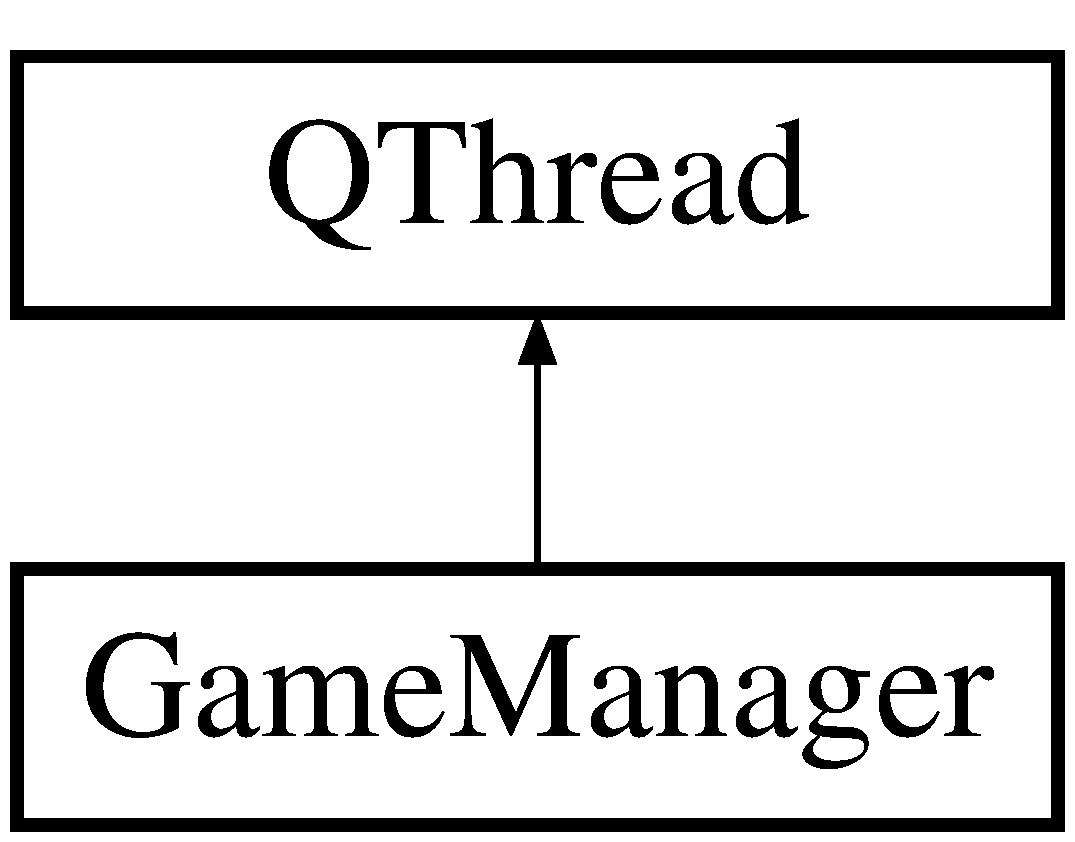
\includegraphics[height=2.000000cm]{classGameManager}
\end{center}
\end{figure}
\subsection*{Classes}
\begin{DoxyCompactItemize}
\item 
struct \hyperlink{structGameManager_1_1AIPlayer}{A\-I\-Player}
\begin{DoxyCompactList}\small\item\em The \hyperlink{classAI}{A\-I} struct Contains a reference to a player which is of type ai and if the ai player has calculated its next move. \end{DoxyCompactList}\end{DoxyCompactItemize}
\subsection*{Signals}
\begin{DoxyCompactItemize}
\item 
\hypertarget{classGameManager_a441d3c2600884f3c315a9c5d3db9066d}{void {\bfseries Play\-Input\-Error\-Sound} ()}\label{classGameManager_a441d3c2600884f3c315a9c5d3db9066d}

\item 
\hypertarget{classGameManager_aa6b2e8ebbbeee51512e865d73342cdce}{void {\bfseries Play\-Input\-Accept\-Sound} ()}\label{classGameManager_aa6b2e8ebbbeee51512e865d73342cdce}

\item 
\hypertarget{classGameManager_aba92c2301c45b00826365149ae8c4844}{void \hyperlink{classGameManager_aba92c2301c45b00826365149ae8c4844}{Turn\-Finished} ()}\label{classGameManager_aba92c2301c45b00826365149ae8c4844}

\begin{DoxyCompactList}\small\item\em Turn\-Finished emitted when players turn finishes. \end{DoxyCompactList}\item 
\hypertarget{classGameManager_a46ecd98b835abec58ea2b716b600c453}{void \hyperlink{classGameManager_a46ecd98b835abec58ea2b716b600c453}{Player\-Won} ()}\label{classGameManager_a46ecd98b835abec58ea2b716b600c453}

\begin{DoxyCompactList}\small\item\em Player\-Won emitted when a player won. \end{DoxyCompactList}\end{DoxyCompactItemize}
\subsection*{Public Member Functions}
\begin{DoxyCompactItemize}
\item 
\hypertarget{classGameManager_aa0e2424dc1a39d380e5b6605b179bf05}{\hyperlink{classGameManager_aa0e2424dc1a39d380e5b6605b179bf05}{Game\-Manager} ()}\label{classGameManager_aa0e2424dc1a39d380e5b6605b179bf05}

\begin{DoxyCompactList}\small\item\em \hyperlink{classGameManager}{Game\-Manager}. \end{DoxyCompactList}\item 
\hyperlink{classGameManager_a80046eb2f443289f0ba1b3fa1272470a}{Game\-Manager} (\hyperlink{classGameData}{Game\-Data} $\ast$data)
\begin{DoxyCompactList}\small\item\em \hyperlink{classGameManager}{Game\-Manager}. \end{DoxyCompactList}\item 
\hypertarget{classGameManager_aaae63e38e358379c1fe507c5197a8435}{virtual \hyperlink{classGameManager_aaae63e38e358379c1fe507c5197a8435}{$\sim$\-Game\-Manager} ()}\label{classGameManager_aaae63e38e358379c1fe507c5197a8435}

\begin{DoxyCompactList}\small\item\em $\sim$\-Game\-Manager \end{DoxyCompactList}\item 
\hypertarget{classGameManager_abbde8090c24ca199815ba1e85059c96f}{virtual void \hyperlink{classGameManager_abbde8090c24ca199815ba1e85059c96f}{run} ()}\label{classGameManager_abbde8090c24ca199815ba1e85059c96f}

\begin{DoxyCompactList}\small\item\em run override of the Q\-Thread run \end{DoxyCompactList}\item 
const \hyperlink{classGameData}{Game\-Data} $\ast$ \hyperlink{classGameManager_ae6075cdc12a4b98aeddc4cda20854393}{Get\-Game\-Data} () const 
\begin{DoxyCompactList}\small\item\em Get\-Game\-Data. \end{DoxyCompactList}\item 
\hypertarget{classGameManager_a3af49a72977052275a1217c5018c737f}{void {\bfseries Start\-Game} ()}\label{classGameManager_a3af49a72977052275a1217c5018c737f}

\item 
\hypertarget{classGameManager_a6f108cd9cdd0cf101d19a151e5e76a26}{void {\bfseries Pause\-Game} ()}\label{classGameManager_a6f108cd9cdd0cf101d19a151e5e76a26}

\item 
\hypertarget{classGameManager_ac756f69d83f34849ed763c7de6b2d47f}{void {\bfseries Suspend\-Processing\-Loop} ()}\label{classGameManager_ac756f69d83f34849ed763c7de6b2d47f}

\item 
\hypertarget{classGameManager_a4e3d2ab486b782641640fb82b77963f2}{void \hyperlink{classGameManager_a4e3d2ab486b782641640fb82b77963f2}{Stop\-Game\-Manager\-Thread} ()}\label{classGameManager_a4e3d2ab486b782641640fb82b77963f2}

\begin{DoxyCompactList}\small\item\em Stop sets the boolean to end the Main processing thread when the user quits the game. \end{DoxyCompactList}\item 
void \hyperlink{classGameManager_ade855b10bc61465dfdfb458cf624cf97}{Input\-Confirmation\-Detected} (\hyperlink{structVector2}{Vector2} pos)
\begin{DoxyCompactList}\small\item\em Input\-Confirmation\-Detected. \end{DoxyCompactList}\item 
bool \hyperlink{classGameManager_ab5e866fc01d4d612cd1f84de0df4653f}{Make\-Move} (\hyperlink{structVector3}{Vector3} pos)  throw (\-Playing\-Field\-::\-Field\-Exeptions, std\-::out\-\_\-of\-\_\-range)
\begin{DoxyCompactList}\small\item\em Tries to Occupy the given position , adds the move to the history, checks if the player won ( return true if won), switches currentplayer, and sends out event that a move is done. \end{DoxyCompactList}\end{DoxyCompactItemize}


\subsection{Detailed Description}
The \hyperlink{classGameManager}{Game\-Manager} class Handles the game loop logic in a thread. 

\begin{DoxyAuthor}{Author}
Nils Brandt 

Alexander Luedke
\end{DoxyAuthor}
\begin{DoxyDate}{Date}
08. August 2016
\end{DoxyDate}
\begin{DoxyVersion}{Version}
1.\-0 Add Documentation 
\end{DoxyVersion}


\subsection{Constructor \& Destructor Documentation}
\hypertarget{classGameManager_a80046eb2f443289f0ba1b3fa1272470a}{\index{Game\-Manager@{Game\-Manager}!Game\-Manager@{Game\-Manager}}
\index{Game\-Manager@{Game\-Manager}!GameManager@{Game\-Manager}}
\subsubsection[{Game\-Manager}]{\setlength{\rightskip}{0pt plus 5cm}Game\-Manager\-::\-Game\-Manager (
\begin{DoxyParamCaption}
\item[{{\bf Game\-Data} $\ast$}]{data}
\end{DoxyParamCaption}
)}}\label{classGameManager_a80046eb2f443289f0ba1b3fa1272470a}


\hyperlink{classGameManager}{Game\-Manager}. 


\begin{DoxyParams}{Parameters}
{\em data} & \\
\hline
\end{DoxyParams}


\subsection{Member Function Documentation}
\hypertarget{classGameManager_ae6075cdc12a4b98aeddc4cda20854393}{\index{Game\-Manager@{Game\-Manager}!Get\-Game\-Data@{Get\-Game\-Data}}
\index{Get\-Game\-Data@{Get\-Game\-Data}!GameManager@{Game\-Manager}}
\subsubsection[{Get\-Game\-Data}]{\setlength{\rightskip}{0pt plus 5cm}const {\bf Game\-Data} $\ast$ Game\-Manager\-::\-Get\-Game\-Data (
\begin{DoxyParamCaption}
{}
\end{DoxyParamCaption}
) const}}\label{classGameManager_ae6075cdc12a4b98aeddc4cda20854393}


Get\-Game\-Data. 

\begin{DoxyReturn}{Returns}

\end{DoxyReturn}
\hypertarget{classGameManager_ade855b10bc61465dfdfb458cf624cf97}{\index{Game\-Manager@{Game\-Manager}!Input\-Confirmation\-Detected@{Input\-Confirmation\-Detected}}
\index{Input\-Confirmation\-Detected@{Input\-Confirmation\-Detected}!GameManager@{Game\-Manager}}
\subsubsection[{Input\-Confirmation\-Detected}]{\setlength{\rightskip}{0pt plus 5cm}void Game\-Manager\-::\-Input\-Confirmation\-Detected (
\begin{DoxyParamCaption}
\item[{{\bf Vector2}}]{pos}
\end{DoxyParamCaption}
)}}\label{classGameManager_ade855b10bc61465dfdfb458cf624cf97}


Input\-Confirmation\-Detected. 


\begin{DoxyParams}{Parameters}
{\em pos} & \\
\hline
\end{DoxyParams}
\hypertarget{classGameManager_ab5e866fc01d4d612cd1f84de0df4653f}{\index{Game\-Manager@{Game\-Manager}!Make\-Move@{Make\-Move}}
\index{Make\-Move@{Make\-Move}!GameManager@{Game\-Manager}}
\subsubsection[{Make\-Move}]{\setlength{\rightskip}{0pt plus 5cm}bool Game\-Manager\-::\-Make\-Move (
\begin{DoxyParamCaption}
\item[{{\bf Vector3}}]{pos}
\end{DoxyParamCaption}
) throw  {\bf Playing\-Field\-::\-Field\-Exeptions}, std\-::out\-\_\-of\-\_\-range) }}\label{classGameManager_ab5e866fc01d4d612cd1f84de0df4653f}


Tries to Occupy the given position , adds the move to the history, checks if the player won ( return true if won), switches currentplayer, and sends out event that a move is done. 


\begin{DoxyParams}{Parameters}
{\em pos} & \\
\hline
\end{DoxyParams}
\begin{DoxyReturn}{Returns}
true if the player just won the game 
\end{DoxyReturn}

\hypertarget{classGameView}{\section{Game\-View Class Reference}
\label{classGameView}\index{Game\-View@{Game\-View}}
}


The \hyperlink{classGameView}{Game\-View} class.  




{\ttfamily \#include $<$Game\-View.\-h$>$}

Inheritance diagram for Game\-View\-:\begin{figure}[H]
\begin{center}
\leavevmode
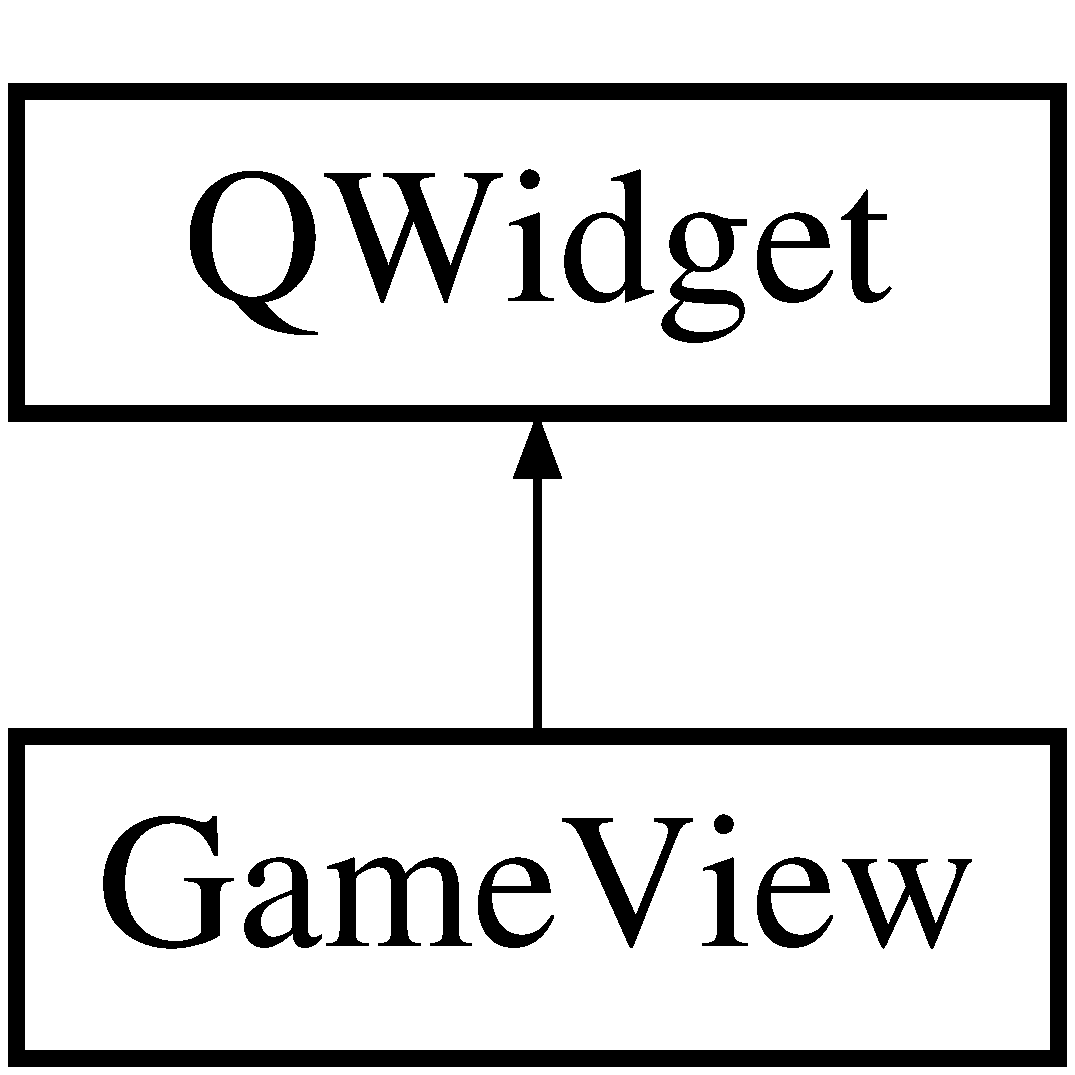
\includegraphics[height=2.000000cm]{classGameView}
\end{center}
\end{figure}
\subsection*{Signals}
\begin{DoxyCompactItemize}
\item 
void \hyperlink{classGameView_a5901d54c9767a75549860cc5b511fcd5}{Game\-Ended} (\hyperlink{classGameData}{Game\-Data} $\ast$data)
\begin{DoxyCompactList}\small\item\em Game\-Ended Called when leave button pressed to go back to menu screen. \end{DoxyCompactList}\item 
\hypertarget{classGameView_a2d1aa868abc05055e5be27040660f7f0}{void \hyperlink{classGameView_a2d1aa868abc05055e5be27040660f7f0}{Pause\-Menu} ()}\label{classGameView_a2d1aa868abc05055e5be27040660f7f0}

\begin{DoxyCompactList}\small\item\em \hyperlink{classPauseMenu}{Pause\-Menu}. \end{DoxyCompactList}\end{DoxyCompactItemize}
\subsection*{Public Member Functions}
\begin{DoxyCompactItemize}
\item 
\hypertarget{classGameView_a6f41d09f51d2abd6abb3b99e5da8ef6f}{{\bfseries Game\-View} (Q\-Widget $\ast$parent=0)}\label{classGameView_a6f41d09f51d2abd6abb3b99e5da8ef6f}

\item 
\hypertarget{classGameView_ae2f4618068a746a97c33859a7550640e}{{\bfseries Game\-View} (\hyperlink{classGameData}{Game\-Data} $\ast$data, Q\-Widget $\ast$parent=0)}\label{classGameView_ae2f4618068a746a97c33859a7550640e}

\item 
\hypertarget{classGameView_aef16847b30bf78a6ecc0888ab1157c8b}{\hyperlink{classGameVisualizer}{Game\-Visualizer} $\ast$ {\bfseries Get\-Visualizer} () const }\label{classGameView_aef16847b30bf78a6ecc0888ab1157c8b}

\item 
\hypertarget{classGameView_a7372d6130ea98db65d8dffc0c4c6989e}{\hyperlink{classGameData}{Game\-Data} $\ast$ {\bfseries Get\-Game\-Data} () const }\label{classGameView_a7372d6130ea98db65d8dffc0c4c6989e}

\item 
\hypertarget{classGameView_a6ecf68723625fae0f3f6301040b166fe}{void {\bfseries Init\-Game} (\hyperlink{classGameData}{Game\-Data} $\ast$data)}\label{classGameView_a6ecf68723625fae0f3f6301040b166fe}

\item 
\hypertarget{classGameView_abd2ab0306c7ce339f7d2d994f21f9f7d}{void {\bfseries Start\-Game} ()}\label{classGameView_abd2ab0306c7ce339f7d2d994f21f9f7d}

\item 
\hypertarget{classGameView_a2b977bd2bd50b851438230f7c4a4ac93}{void {\bfseries Pause\-Game} ()}\label{classGameView_a2b977bd2bd50b851438230f7c4a4ac93}

\item 
\hypertarget{classGameView_a2a1634628f3c981462f54c6c1f18ec6d}{void {\bfseries Play\-Accept\-Sound} ()}\label{classGameView_a2a1634628f3c981462f54c6c1f18ec6d}

\item 
\hypertarget{classGameView_a0bc73aeff44e7e52bd1d73a21dd6a7f2}{void {\bfseries Play\-Error\-Sound} ()}\label{classGameView_a0bc73aeff44e7e52bd1d73a21dd6a7f2}

\item 
\hypertarget{classGameView_a92b306e86ed8fe682763050be4edf254}{void {\bfseries Show\-Game\-Input\-View} ()}\label{classGameView_a92b306e86ed8fe682763050be4edf254}

\item 
\hypertarget{classGameView_a29cba4e6e6963b659f3cb2acbdfc3fe1}{void {\bfseries Show\-Winner} ()}\label{classGameView_a29cba4e6e6963b659f3cb2acbdfc3fe1}

\item 
\hypertarget{classGameView_a3e06ec8f766005c4aac0d572559fc9ed}{void \hyperlink{classGameView_a3e06ec8f766005c4aac0d572559fc9ed}{Game\-Finished} ()}\label{classGameView_a3e06ec8f766005c4aac0d572559fc9ed}

\begin{DoxyCompactList}\small\item\em Game\-Finished Called if a player won to stop the gamelogic thread and show leave button. \end{DoxyCompactList}\item 
\hypertarget{classGameView_a157ac747504394587761ac30a79b9597}{void \hyperlink{classGameView_a157ac747504394587761ac30a79b9597}{End\-Game} ()}\label{classGameView_a157ac747504394587761ac30a79b9597}

\begin{DoxyCompactList}\small\item\em End\-Game called from leave button calls Game\-Ended. \end{DoxyCompactList}\item 
\hypertarget{classGameView_a5d6aac6e502ec51285f03ba51da00886}{void {\bfseries change\-Event} (Q\-Event $\ast$event)}\label{classGameView_a5d6aac6e502ec51285f03ba51da00886}

\end{DoxyCompactItemize}


\subsection{Detailed Description}
The \hyperlink{classGameView}{Game\-View} class. 

\begin{DoxyAuthor}{Author}
Nils Brandt 

Alexander Luedke
\end{DoxyAuthor}
\begin{DoxyDate}{Date}
08. August 2016
\end{DoxyDate}
\begin{DoxyVersion}{Version}
1.\-0 Add Documentation 
\end{DoxyVersion}


\subsection{Member Function Documentation}
\hypertarget{classGameView_a5901d54c9767a75549860cc5b511fcd5}{\index{Game\-View@{Game\-View}!Game\-Ended@{Game\-Ended}}
\index{Game\-Ended@{Game\-Ended}!GameView@{Game\-View}}
\subsubsection[{Game\-Ended}]{\setlength{\rightskip}{0pt plus 5cm}void Game\-View\-::\-Game\-Ended (
\begin{DoxyParamCaption}
\item[{{\bf Game\-Data} $\ast$}]{data}
\end{DoxyParamCaption}
)\hspace{0.3cm}{\ttfamily [signal]}}}\label{classGameView_a5901d54c9767a75549860cc5b511fcd5}


Game\-Ended Called when leave button pressed to go back to menu screen. 


\begin{DoxyParams}{Parameters}
{\em data} & gamedata after game ended \\
\hline
\end{DoxyParams}

\hypertarget{classGameView2D}{\section{Game\-View2\-D Class Reference}
\label{classGameView2D}\index{Game\-View2\-D@{Game\-View2\-D}}
}


The \hyperlink{classGameView2D}{Game\-View2\-D} class.  




{\ttfamily \#include $<$Game\-View2\-D.\-h$>$}

Inheritance diagram for Game\-View2\-D\-:\begin{figure}[H]
\begin{center}
\leavevmode
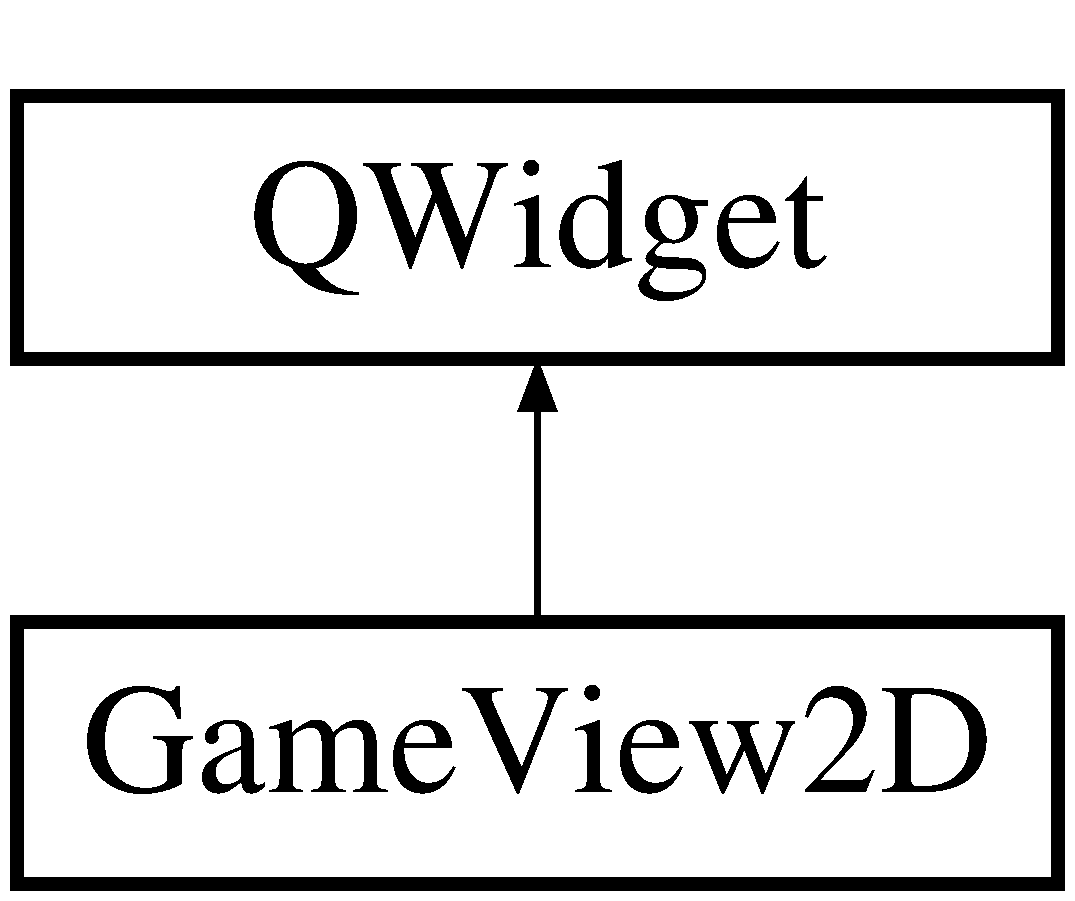
\includegraphics[height=2.000000cm]{classGameView2D}
\end{center}
\end{figure}
\subsection*{Public Member Functions}
\begin{DoxyCompactItemize}
\item 
\hypertarget{classGameView2D_ade0d3e85d2385f952db7a5a72dcc34e3}{{\bfseries Game\-View2\-D} (\hyperlink{classGameManager}{Game\-Manager} $\ast$manager, Q\-Widget $\ast$parent=0)}\label{classGameView2D_ade0d3e85d2385f952db7a5a72dcc34e3}

\item 
\hypertarget{classGameView2D_a2599584223096c30f37ed12566ccea32}{\hyperlink{classGraphicsSlot2D}{Graphics\-Slot2\-D} $\ast$ {\bfseries Get\-Rect} (\hyperlink{structVector3}{Vector3} vec)}\label{classGameView2D_a2599584223096c30f37ed12566ccea32}

\item 
\hypertarget{classGameView2D_aa30c0b87cc0c44a68a9f30b5e9e22ea4}{void \hyperlink{classGameView2D_aa30c0b87cc0c44a68a9f30b5e9e22ea4}{Clear\-Grid} ()}\label{classGameView2D_aa30c0b87cc0c44a68a9f30b5e9e22ea4}

\begin{DoxyCompactList}\small\item\em To clear the grid. \end{DoxyCompactList}\item 
\hypertarget{classGameView2D_aaf46ebd46da445c65fb1d54e805b7d9c}{void {\bfseries Recalculate\-Grid} ()}\label{classGameView2D_aaf46ebd46da445c65fb1d54e805b7d9c}

\item 
\hypertarget{classGameView2D_ad826ed1dccdcae1508693615e20df95e}{void \hyperlink{classGameView2D_ad826ed1dccdcae1508693615e20df95e}{View\-Update} ()}\label{classGameView2D_ad826ed1dccdcae1508693615e20df95e}

\begin{DoxyCompactList}\small\item\em View\-Update. \end{DoxyCompactList}\end{DoxyCompactItemize}


\subsection{Detailed Description}
The \hyperlink{classGameView2D}{Game\-View2\-D} class. 

\begin{DoxyAuthor}{Author}
Nils Brandt 

Alexander Luedke
\end{DoxyAuthor}
\begin{DoxyDate}{Date}
08. August 2016
\end{DoxyDate}
\begin{DoxyVersion}{Version}
1.\-0 Add Documentation 
\end{DoxyVersion}

\hypertarget{classGameView3D}{\section{Game\-View3\-D Class Reference}
\label{classGameView3D}\index{Game\-View3\-D@{Game\-View3\-D}}
}


The \hyperlink{classGameView3D}{Game\-View3\-D} class.  




{\ttfamily \#include $<$Game\-View3\-D.\-h$>$}

Inheritance diagram for Game\-View3\-D\-:\begin{figure}[H]
\begin{center}
\leavevmode
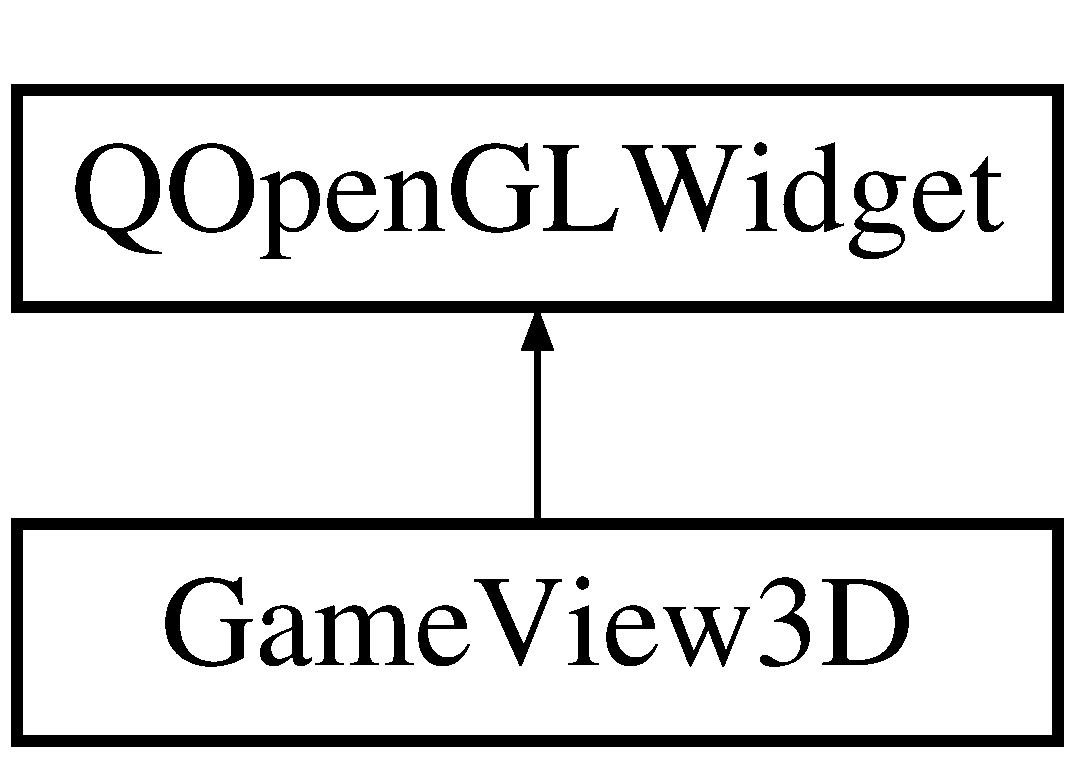
\includegraphics[height=2.000000cm]{classGameView3D}
\end{center}
\end{figure}
\subsection*{Signals}
\begin{DoxyCompactItemize}
\item 
\hypertarget{classGameView3D_ada434861732fe261a9a7958de4fb5f2e}{void {\bfseries Input\-Submit} (\hyperlink{structVector2}{Vector2} pos)}\label{classGameView3D_ada434861732fe261a9a7958de4fb5f2e}

\end{DoxyCompactItemize}
\subsection*{Public Member Functions}
\begin{DoxyCompactItemize}
\item 
\hypertarget{classGameView3D_aa2a60cd38325c7a4ec92909d2efe7a80}{{\bfseries Game\-View3\-D} (Q\-Widget $\ast$parent=0)}\label{classGameView3D_aa2a60cd38325c7a4ec92909d2efe7a80}

\item 
\hypertarget{classGameView3D_a447292a1846348584fea8cbd2392d1dd}{{\bfseries Game\-View3\-D} (\hyperlink{classGameManager}{Game\-Manager} $\ast$gm, Q\-Widget $\ast$parent=0)}\label{classGameView3D_a447292a1846348584fea8cbd2392d1dd}

\item 
\hypertarget{classGameView3D_a9662a858540b5fcc1a80d78cd0a0aa2a}{void {\bfseries Clean\-Up} ()}\label{classGameView3D_a9662a858540b5fcc1a80d78cd0a0aa2a}

\end{DoxyCompactItemize}
\subsection*{Protected Member Functions}
\begin{DoxyCompactItemize}
\item 
\hypertarget{classGameView3D_ae077404d42f477162b3540da397a8ad4}{void {\bfseries send\-M\-V\-P} (G\-Luint program\-I\-D)}\label{classGameView3D_ae077404d42f477162b3540da397a8ad4}

\item 
\hypertarget{classGameView3D_ae6db5f0d969ca92280e4dc6c7092e11e}{virtual void {\bfseries initialize\-G\-L} ()}\label{classGameView3D_ae6db5f0d969ca92280e4dc6c7092e11e}

\item 
\hypertarget{classGameView3D_ad69d664507756b94cc64ab65581528c4}{virtual void {\bfseries paint\-G\-L} ()}\label{classGameView3D_ad69d664507756b94cc64ab65581528c4}

\item 
\hypertarget{classGameView3D_ad08f12d05b40dbbb42172783fb4ffe5f}{virtual void {\bfseries resize\-G\-L} (int w, int h)}\label{classGameView3D_ad08f12d05b40dbbb42172783fb4ffe5f}

\item 
\hypertarget{classGameView3D_abeb74e91cd820d7af1e62c714fc1864f}{void {\bfseries key\-Press\-Event} (Q\-Key\-Event $\ast$event)}\label{classGameView3D_abeb74e91cd820d7af1e62c714fc1864f}

\item 
\hypertarget{classGameView3D_a2a66712712d355039299efb5513fbeb2}{void {\bfseries mouse\-Press\-Event} (Q\-Mouse\-Event $\ast$event)}\label{classGameView3D_a2a66712712d355039299efb5513fbeb2}

\item 
\hypertarget{classGameView3D_a16eb2fd0448d2f50b1c5287f86ac9437}{void {\bfseries mouse\-Move\-Event} (Q\-Mouse\-Event $\ast$event)}\label{classGameView3D_a16eb2fd0448d2f50b1c5287f86ac9437}

\item 
\hypertarget{classGameView3D_aa4d6e119510fc03c95d52282579ca8ed}{bool {\bfseries Cast\-Ray} (Q\-Point m\-\_\-current\-Mouse\-Pos)}\label{classGameView3D_aa4d6e119510fc03c95d52282579ca8ed}

\item 
\hypertarget{classGameView3D_a31d588b55fd79e52732a28ccd196733c}{void {\bfseries Create\-Line} (glm\-::vec3 start, glm\-::vec3 end, G\-Luint \&Vertex\-Array\-I\-D\-Line)}\label{classGameView3D_a31d588b55fd79e52732a28ccd196733c}

\item 
\hypertarget{classGameView3D_a5e9b5ac73aaa4fedf3bbbec02544c184}{void {\bfseries Draw\-Line} (glm\-::vec3 start, glm\-::vec3 end)}\label{classGameView3D_a5e9b5ac73aaa4fedf3bbbec02544c184}

\item 
\hypertarget{classGameView3D_aa96228c70d0a93420abef7687518f809}{void {\bfseries Screen\-Pos\-To\-World\-Ray} (int mouse\-X, int mouse\-Y, int screen\-Width, int screen\-Height, glm\-::mat4 View\-Matrix, glm\-::mat4 Projection\-Matrix, glm\-::vec3 \&out\-\_\-origin, glm\-::vec3 \&out\-\_\-direction)}\label{classGameView3D_aa96228c70d0a93420abef7687518f809}

\item 
\hypertarget{classGameView3D_a301575899b1763b95a99e4c386f9356d}{bool {\bfseries Test\-Ray\-O\-B\-B\-Intersection} (glm\-::vec3 ray\-\_\-origin, glm\-::vec3 ray\-\_\-direction, glm\-::vec3 aabb\-\_\-min, glm\-::vec3 aabb\-\_\-max, glm\-::mat4 Model\-Matrix, float \&intersection\-\_\-distance)}\label{classGameView3D_a301575899b1763b95a99e4c386f9356d}

\end{DoxyCompactItemize}


\subsection{Detailed Description}
The \hyperlink{classGameView3D}{Game\-View3\-D} class. 

\begin{DoxyAuthor}{Author}
Nils Brandt 

Alexander Luedke
\end{DoxyAuthor}
\begin{DoxyDate}{Date}
08. August 2016
\end{DoxyDate}
\begin{DoxyVersion}{Version}
1.\-0 Add Documentation 
\end{DoxyVersion}

\hypertarget{classGameVisualizer}{\section{Game\-Visualizer Class Reference}
\label{classGameVisualizer}\index{Game\-Visualizer@{Game\-Visualizer}}
}


The \hyperlink{classGameVisualizer}{Game\-Visualizer} class.  




{\ttfamily \#include $<$Game\-Visualizer.\-h$>$}

Inheritance diagram for Game\-Visualizer\-:\begin{figure}[H]
\begin{center}
\leavevmode
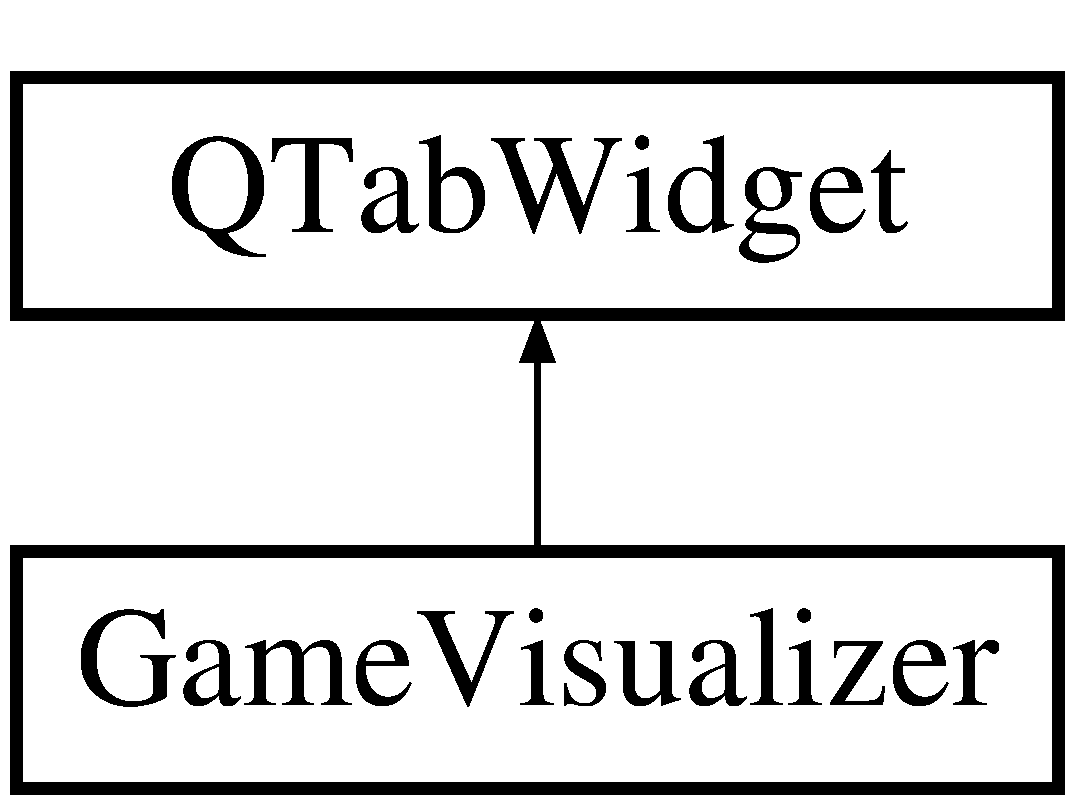
\includegraphics[height=2.000000cm]{classGameVisualizer}
\end{center}
\end{figure}
\subsection*{Signals}
\begin{DoxyCompactItemize}
\item 
\hypertarget{classGameVisualizer_abb8ff4568ee3c5ed30cbc2df3d32df84}{void {\bfseries Input\-Detected} (\hyperlink{structVector2}{Vector2} pos)}\label{classGameVisualizer_abb8ff4568ee3c5ed30cbc2df3d32df84}

\end{DoxyCompactItemize}
\subsection*{Public Member Functions}
\begin{DoxyCompactItemize}
\item 
\hypertarget{classGameVisualizer_ac6e640e1cfa0162d63158670741d9485}{{\bfseries Game\-Visualizer} (\hyperlink{classGameManager}{Game\-Manager} $\ast$manager, Q\-Widget $\ast$parent=0)}\label{classGameVisualizer_ac6e640e1cfa0162d63158670741d9485}

\item 
\hypertarget{classGameVisualizer_ac68aa47882b34f28427e3e161f677f9d}{void {\bfseries Update\-Views} ()}\label{classGameVisualizer_ac68aa47882b34f28427e3e161f677f9d}

\item 
\hypertarget{classGameVisualizer_a5fb41e30e67173d36f3769d804130b19}{void {\bfseries Update\-View2\-D} ()}\label{classGameVisualizer_a5fb41e30e67173d36f3769d804130b19}

\item 
\hypertarget{classGameVisualizer_aee1fac4e1657fb4be1fa61f563b02d32}{void {\bfseries Update\-View3\-D} ()}\label{classGameVisualizer_aee1fac4e1657fb4be1fa61f563b02d32}

\item 
\hypertarget{classGameVisualizer_a3a8cf6d067d4d0272c1b3b60f44f8d1c}{void {\bfseries Game\-Changed} ()}\label{classGameVisualizer_a3a8cf6d067d4d0272c1b3b60f44f8d1c}

\end{DoxyCompactItemize}


\subsection{Detailed Description}
The \hyperlink{classGameVisualizer}{Game\-Visualizer} class. 

\begin{DoxyAuthor}{Author}
Nils Brandt 

Alexander Luedke
\end{DoxyAuthor}
\begin{DoxyDate}{Date}
08. August 2016
\end{DoxyDate}
\begin{DoxyVersion}{Version}
1.\-0 Add Documentation 
\end{DoxyVersion}

\hypertarget{classGraphicsSlot2D}{\section{Graphics\-Slot2\-D Class Reference}
\label{classGraphicsSlot2D}\index{Graphics\-Slot2\-D@{Graphics\-Slot2\-D}}
}


The \hyperlink{classGraphicsSlot2D}{Graphics\-Slot2\-D} class.  




{\ttfamily \#include $<$Graphics\-Slot2d.\-h$>$}

Inheritance diagram for Graphics\-Slot2\-D\-:\begin{figure}[H]
\begin{center}
\leavevmode
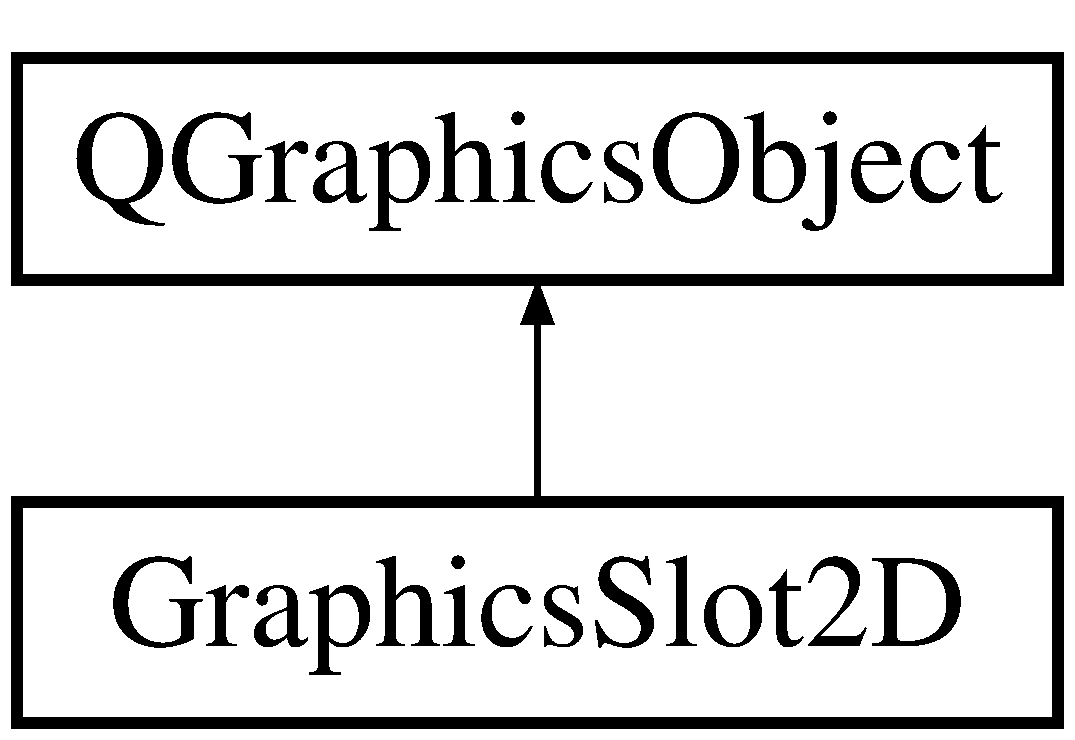
\includegraphics[height=2.000000cm]{classGraphicsSlot2D}
\end{center}
\end{figure}
\subsection*{Signals}
\begin{DoxyCompactItemize}
\item 
\hypertarget{classGraphicsSlot2D_a1cca679459243a836ace0c4aca3923e8}{void {\bfseries Clicked\-Signal} (\hyperlink{classGraphicsSlot2D}{Graphics\-Slot2\-D} $\ast$ref)}\label{classGraphicsSlot2D_a1cca679459243a836ace0c4aca3923e8}

\end{DoxyCompactItemize}
\subsection*{Public Member Functions}
\begin{DoxyCompactItemize}
\item 
\hypertarget{classGraphicsSlot2D_a727b75d36aeec94cb0ea7ba87d2b4018}{{\bfseries Graphics\-Slot2\-D} (float x, float y, float width, float height, Q\-Color color=Qt\-::white, Q\-Graphics\-Item $\ast$parent=0)}\label{classGraphicsSlot2D_a727b75d36aeec94cb0ea7ba87d2b4018}

\item 
\hypertarget{classGraphicsSlot2D_a91bbc858f2f966d88f5dfc3a9255b262}{virtual Q\-Rect\-F {\bfseries bounding\-Rect} () const Q\-\_\-\-D\-E\-C\-L\-\_\-\-O\-V\-E\-R\-R\-I\-D\-E}\label{classGraphicsSlot2D_a91bbc858f2f966d88f5dfc3a9255b262}

\item 
\hypertarget{classGraphicsSlot2D_acb9706b9269de9e2a8221b34d117e66e}{Q\-Color {\bfseries Get\-Color} () const }\label{classGraphicsSlot2D_acb9706b9269de9e2a8221b34d117e66e}

\item 
\hypertarget{classGraphicsSlot2D_aa505d921ccd7d8e92ee2b5d028b768c4}{void {\bfseries Set\-Size} (float x, float y)}\label{classGraphicsSlot2D_aa505d921ccd7d8e92ee2b5d028b768c4}

\item 
\hypertarget{classGraphicsSlot2D_a6e7ccd8e16d8cb8b558eaddfbe4ac3b5}{void {\bfseries Set\-Color} (Q\-Color color)}\label{classGraphicsSlot2D_a6e7ccd8e16d8cb8b558eaddfbe4ac3b5}

\item 
\hypertarget{classGraphicsSlot2D_a28747f4550d08b4fe2853d820b936127}{virtual void {\bfseries paint} (Q\-Painter $\ast$painter, const Q\-Style\-Option\-Graphics\-Item $\ast$option, Q\-Widget $\ast$widget=Q\-\_\-\-N\-U\-L\-L\-P\-T\-R) Q\-\_\-\-D\-E\-C\-L\-\_\-\-O\-V\-E\-R\-R\-I\-D\-E}\label{classGraphicsSlot2D_a28747f4550d08b4fe2853d820b936127}

\item 
\hypertarget{classGraphicsSlot2D_acef178475ff7ac3d225e2fa255ceef0d}{void {\bfseries mouse\-Press\-Event} (Q\-Graphics\-Scene\-Mouse\-Event $\ast$event) Q\-\_\-\-D\-E\-C\-L\-\_\-\-O\-V\-E\-R\-R\-I\-D\-E}\label{classGraphicsSlot2D_acef178475ff7ac3d225e2fa255ceef0d}

\end{DoxyCompactItemize}


\subsection{Detailed Description}
The \hyperlink{classGraphicsSlot2D}{Graphics\-Slot2\-D} class. 

The documentation for this class was generated from the following files\-:\begin{DoxyCompactItemize}
\item 
/home/alex/source\-Code/git\-Project/beleg\-Arbeit\-E\-M\-M\-S/project\-Sogo/include/gui/Graphics\-Slot2d.\-h\item 
/home/alex/source\-Code/git\-Project/beleg\-Arbeit\-E\-M\-M\-S/project\-Sogo/build-\/sogo\-App-\/\-Desktop\-\_\-\-Qt\-\_\-5\-\_\-6\-\_\-0\-\_\-\-G\-C\-C\-\_\-64bit-\/\-Debug/moc\-\_\-\-Graphics\-Slot2d.\-cpp\item 
/home/alex/source\-Code/git\-Project/beleg\-Arbeit\-E\-M\-M\-S/project\-Sogo/src/gui/Graphics\-Slot2d.\-cpp\end{DoxyCompactItemize}

\hypertarget{classHighscoreMenu}{\section{Highscore\-Menu Class Reference}
\label{classHighscoreMenu}\index{Highscore\-Menu@{Highscore\-Menu}}
}


The \hyperlink{classHighscoreMenu}{Highscore\-Menu} class.  




{\ttfamily \#include $<$Highscore\-Menu.\-h$>$}

Inheritance diagram for Highscore\-Menu\-:\begin{figure}[H]
\begin{center}
\leavevmode
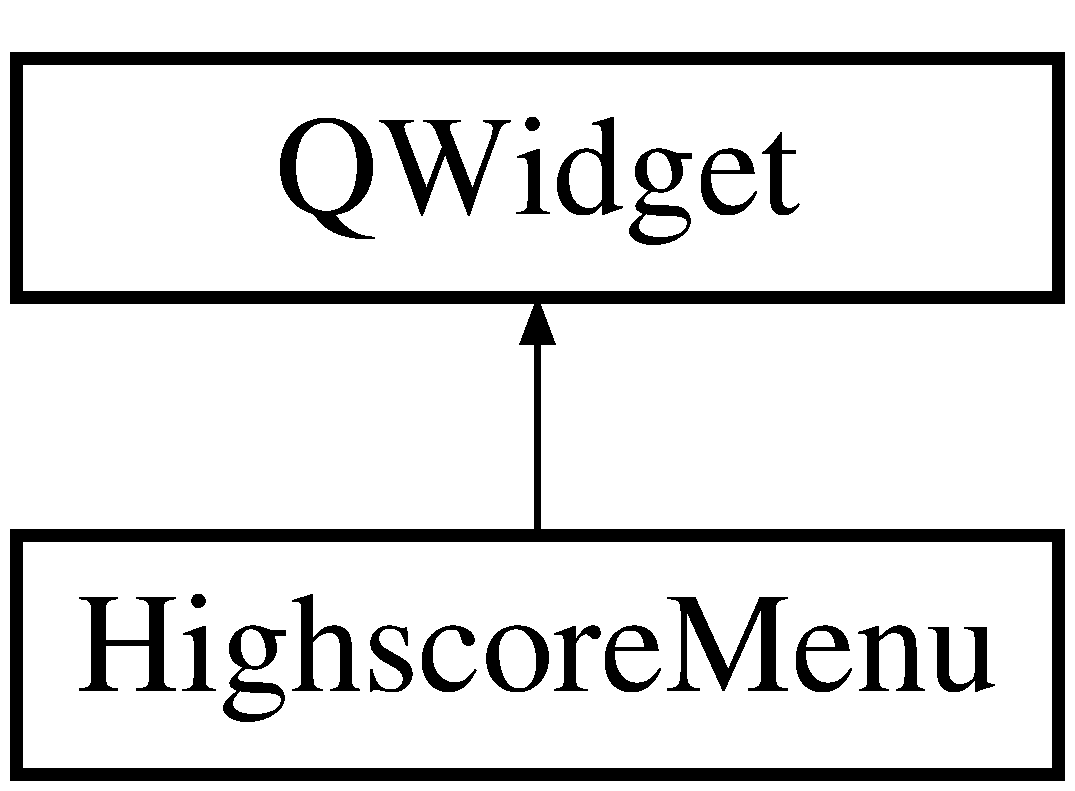
\includegraphics[height=2.000000cm]{classHighscoreMenu}
\end{center}
\end{figure}
\subsection*{Signals}
\begin{DoxyCompactItemize}
\item 
\hypertarget{classHighscoreMenu_acfc660f3078cc3e42a2b0be20f534e59}{void {\bfseries show\-Start\-Menu} ()}\label{classHighscoreMenu_acfc660f3078cc3e42a2b0be20f534e59}

\end{DoxyCompactItemize}
\subsection*{Public Member Functions}
\begin{DoxyCompactItemize}
\item 
\hypertarget{classHighscoreMenu_afffd6ba37985beae539f7d143de2201d}{{\bfseries Highscore\-Menu} (Q\-Widget $\ast$parent=0)}\label{classHighscoreMenu_afffd6ba37985beae539f7d143de2201d}

\item 
\hypertarget{classHighscoreMenu_ad71f69706ab1969e180abc4794f946c9}{void {\bfseries change\-Event} (Q\-Event $\ast$event)}\label{classHighscoreMenu_ad71f69706ab1969e180abc4794f946c9}

\end{DoxyCompactItemize}


\subsection{Detailed Description}
The \hyperlink{classHighscoreMenu}{Highscore\-Menu} class. 

\begin{DoxyAuthor}{Author}
Nils Brandt 

Alexander Luedke
\end{DoxyAuthor}
\begin{DoxyDate}{Date}
08. August 2016
\end{DoxyDate}
\begin{DoxyVersion}{Version}
1.\-0 Add Documentation 
\end{DoxyVersion}

\hypertarget{classHistoryDisplay}{\section{History\-Display Class Reference}
\label{classHistoryDisplay}\index{History\-Display@{History\-Display}}
}


The \hyperlink{classHistoryDisplay}{History\-Display} class.  




{\ttfamily \#include $<$History\-Display.\-h$>$}

Inheritance diagram for History\-Display\-:\begin{figure}[H]
\begin{center}
\leavevmode
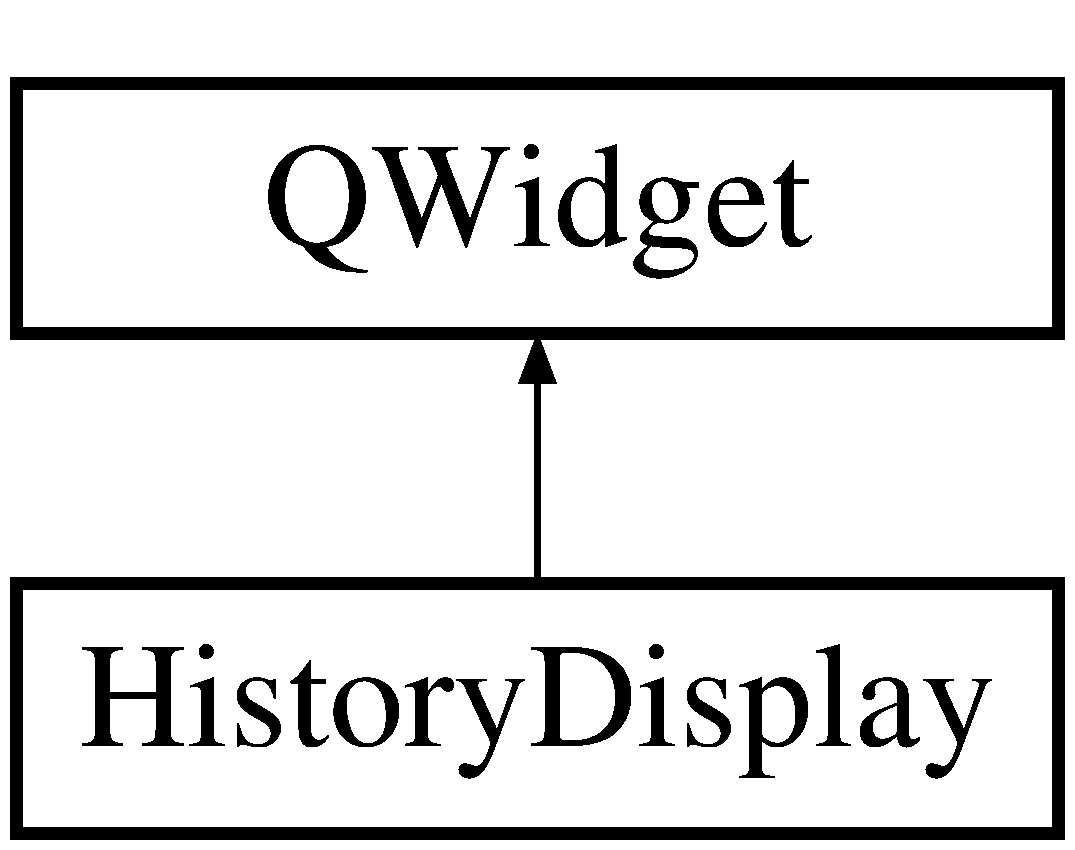
\includegraphics[height=2.000000cm]{classHistoryDisplay}
\end{center}
\end{figure}
\subsection*{Public Member Functions}
\begin{DoxyCompactItemize}
\item 
\hypertarget{classHistoryDisplay_ad4b7962e85e825f2a1e0c90cf1f8e201}{{\bfseries History\-Display} (const \hyperlink{classGameData}{Game\-Data} $\ast$data, Q\-Widget $\ast$parent=0)}\label{classHistoryDisplay_ad4b7962e85e825f2a1e0c90cf1f8e201}

\item 
\hypertarget{classHistoryDisplay_a360a99566c00c9166ad3a0552e0d801e}{void \hyperlink{classHistoryDisplay_a360a99566c00c9166ad3a0552e0d801e}{Update\-History} ()}\label{classHistoryDisplay_a360a99566c00c9166ad3a0552e0d801e}

\begin{DoxyCompactList}\small\item\em Update\-History clears display reevaluates past moves and displays new text. \end{DoxyCompactList}\item 
\hypertarget{classHistoryDisplay_ad3359c47f96baa4747bf7dde034ab222}{void \hyperlink{classHistoryDisplay_ad3359c47f96baa4747bf7dde034ab222}{Redraw\-History} ()}\label{classHistoryDisplay_ad3359c47f96baa4747bf7dde034ab222}

\begin{DoxyCompactList}\small\item\em Redraw\-History clears and redraws history. \end{DoxyCompactList}\item 
void \hyperlink{classHistoryDisplay_a260307ebdade967004f32cf48f877915}{Set\-Display\-Text} (std\-::string entry)
\begin{DoxyCompactList}\small\item\em Display\-Text Called to change the text in the Display box. \end{DoxyCompactList}\item 
\hypertarget{classHistoryDisplay_a8c548187b6eb9152655f20b4f8cae402}{void {\bfseries change\-Event} (Q\-Event $\ast$event)}\label{classHistoryDisplay_a8c548187b6eb9152655f20b4f8cae402}

\end{DoxyCompactItemize}


\subsection{Detailed Description}
The \hyperlink{classHistoryDisplay}{History\-Display} class. 

\subsection{Member Function Documentation}
\hypertarget{classHistoryDisplay_a260307ebdade967004f32cf48f877915}{\index{History\-Display@{History\-Display}!Set\-Display\-Text@{Set\-Display\-Text}}
\index{Set\-Display\-Text@{Set\-Display\-Text}!HistoryDisplay@{History\-Display}}
\subsubsection[{Set\-Display\-Text}]{\setlength{\rightskip}{0pt plus 5cm}void History\-Display\-::\-Set\-Display\-Text (
\begin{DoxyParamCaption}
\item[{std\-::string}]{entry}
\end{DoxyParamCaption}
)}}\label{classHistoryDisplay_a260307ebdade967004f32cf48f877915}


Display\-Text Called to change the text in the Display box. 


\begin{DoxyParams}{Parameters}
{\em entry} & \\
\hline
\end{DoxyParams}


The documentation for this class was generated from the following files\-:\begin{DoxyCompactItemize}
\item 
/home/alex/source\-Code/git\-Project/beleg\-Arbeit\-E\-M\-M\-S/project\-Sogo/include/gui/History\-Display.\-h\item 
/home/alex/source\-Code/git\-Project/beleg\-Arbeit\-E\-M\-M\-S/project\-Sogo/src/gui/History\-Display.\-cpp\end{DoxyCompactItemize}

\hypertarget{classHistorySave}{\section{History\-Save Class Reference}
\label{classHistorySave}\index{History\-Save@{History\-Save}}
}


The \hyperlink{classHistorySave}{History\-Save} class.  




{\ttfamily \#include $<$History\-Save.\-h$>$}

\subsection*{Public Member Functions}
\begin{DoxyCompactItemize}
\item 
\hypertarget{classHistorySave_a1f76c15dd7a3b9e27a8c66897141ee16}{\hyperlink{classHistorySave_a1f76c15dd7a3b9e27a8c66897141ee16}{History\-Save} ()}\label{classHistorySave_a1f76c15dd7a3b9e27a8c66897141ee16}

\begin{DoxyCompactList}\small\item\em \hyperlink{classHistorySave}{History\-Save}. \end{DoxyCompactList}\item 
\hyperlink{classHistorySave_ac0766707b25e837d00e6e4b48bf2860c}{History\-Save} (const \hyperlink{classHistorySave}{History\-Save} \&src)
\begin{DoxyCompactList}\small\item\em \hyperlink{classHistorySave}{History\-Save}. \end{DoxyCompactList}\item 
void \hyperlink{classHistorySave_a4d10cac993d69d8f98f9c32eb7ae4a2d}{Add\-Move} (\hyperlink{structVector3}{Vector3} pos, \hyperlink{classPlayer}{Player} player)
\begin{DoxyCompactList}\small\item\em Add\-Move. \end{DoxyCompactList}\item 
\hypertarget{classHistorySave_a4adce01fc1a4deb3a80d7ac5e3a38860}{void \hyperlink{classHistorySave_a4adce01fc1a4deb3a80d7ac5e3a38860}{Revert\-Last} ()}\label{classHistorySave_a4adce01fc1a4deb3a80d7ac5e3a38860}

\begin{DoxyCompactList}\small\item\em Revert\-Last. \end{DoxyCompactList}\item 
int \hyperlink{classHistorySave_af1f736a6ee2b72f56ac6985e788013a9}{Get\-Move\-Count} () const 
\begin{DoxyCompactList}\small\item\em Get\-Move\-Count. \end{DoxyCompactList}\item 
const Move $\ast$ \hyperlink{classHistorySave_ae04d28f2fa9c879beb2631f318526f3a}{Get\-Move} (int number) const   throw (out\-\_\-of\-\_\-range)
\begin{DoxyCompactList}\small\item\em Get\-Move. \end{DoxyCompactList}\item 
const Move $\ast$ \hyperlink{classHistorySave_ab8c21fe924b58510b9e240b5b5852be2}{Get\-Last\-Move} () const   throw (out\-\_\-of\-\_\-range)
\begin{DoxyCompactList}\small\item\em Get\-Last\-Move. \end{DoxyCompactList}\end{DoxyCompactItemize}


\subsection{Detailed Description}
The \hyperlink{classHistorySave}{History\-Save} class. 

\subsection{Constructor \& Destructor Documentation}
\hypertarget{classHistorySave_ac0766707b25e837d00e6e4b48bf2860c}{\index{History\-Save@{History\-Save}!History\-Save@{History\-Save}}
\index{History\-Save@{History\-Save}!HistorySave@{History\-Save}}
\subsubsection[{History\-Save}]{\setlength{\rightskip}{0pt plus 5cm}History\-Save\-::\-History\-Save (
\begin{DoxyParamCaption}
\item[{const {\bf History\-Save} \&}]{src}
\end{DoxyParamCaption}
)}}\label{classHistorySave_ac0766707b25e837d00e6e4b48bf2860c}


\hyperlink{classHistorySave}{History\-Save}. 


\begin{DoxyParams}{Parameters}
{\em src} & \\
\hline
\end{DoxyParams}


\subsection{Member Function Documentation}
\hypertarget{classHistorySave_a4d10cac993d69d8f98f9c32eb7ae4a2d}{\index{History\-Save@{History\-Save}!Add\-Move@{Add\-Move}}
\index{Add\-Move@{Add\-Move}!HistorySave@{History\-Save}}
\subsubsection[{Add\-Move}]{\setlength{\rightskip}{0pt plus 5cm}void History\-Save\-::\-Add\-Move (
\begin{DoxyParamCaption}
\item[{{\bf Vector3}}]{pos, }
\item[{{\bf Player}}]{player}
\end{DoxyParamCaption}
)}}\label{classHistorySave_a4d10cac993d69d8f98f9c32eb7ae4a2d}


Add\-Move. 


\begin{DoxyParams}{Parameters}
{\em pos} & \\
\hline
{\em player} & \\
\hline
\end{DoxyParams}
\hypertarget{classHistorySave_ab8c21fe924b58510b9e240b5b5852be2}{\index{History\-Save@{History\-Save}!Get\-Last\-Move@{Get\-Last\-Move}}
\index{Get\-Last\-Move@{Get\-Last\-Move}!HistorySave@{History\-Save}}
\subsubsection[{Get\-Last\-Move}]{\setlength{\rightskip}{0pt plus 5cm}const Move$\ast$ History\-Save\-::\-Get\-Last\-Move (
\begin{DoxyParamCaption}
{}
\end{DoxyParamCaption}
) const throw  out\-\_\-of\-\_\-range) \hspace{0.3cm}{\ttfamily [inline]}}}\label{classHistorySave_ab8c21fe924b58510b9e240b5b5852be2}


Get\-Last\-Move. 

\begin{DoxyReturn}{Returns}

\end{DoxyReturn}
\hypertarget{classHistorySave_ae04d28f2fa9c879beb2631f318526f3a}{\index{History\-Save@{History\-Save}!Get\-Move@{Get\-Move}}
\index{Get\-Move@{Get\-Move}!HistorySave@{History\-Save}}
\subsubsection[{Get\-Move}]{\setlength{\rightskip}{0pt plus 5cm}const Move$\ast$ History\-Save\-::\-Get\-Move (
\begin{DoxyParamCaption}
\item[{int}]{number}
\end{DoxyParamCaption}
) const throw  out\-\_\-of\-\_\-range) \hspace{0.3cm}{\ttfamily [inline]}}}\label{classHistorySave_ae04d28f2fa9c879beb2631f318526f3a}


Get\-Move. 


\begin{DoxyParams}{Parameters}
{\em number} & \\
\hline
\end{DoxyParams}
\begin{DoxyReturn}{Returns}

\end{DoxyReturn}
\hypertarget{classHistorySave_af1f736a6ee2b72f56ac6985e788013a9}{\index{History\-Save@{History\-Save}!Get\-Move\-Count@{Get\-Move\-Count}}
\index{Get\-Move\-Count@{Get\-Move\-Count}!HistorySave@{History\-Save}}
\subsubsection[{Get\-Move\-Count}]{\setlength{\rightskip}{0pt plus 5cm}int History\-Save\-::\-Get\-Move\-Count (
\begin{DoxyParamCaption}
{}
\end{DoxyParamCaption}
) const\hspace{0.3cm}{\ttfamily [inline]}}}\label{classHistorySave_af1f736a6ee2b72f56ac6985e788013a9}


Get\-Move\-Count. 

\begin{DoxyReturn}{Returns}

\end{DoxyReturn}


The documentation for this class was generated from the following files\-:\begin{DoxyCompactItemize}
\item 
/home/alex/source\-Code/git\-Project/beleg\-Arbeit\-E\-M\-M\-S/project\-Sogo/include/core/History\-Save.\-h\item 
/home/alex/source\-Code/git\-Project/beleg\-Arbeit\-E\-M\-M\-S/project\-Sogo/src/core/History\-Save.\-cpp\end{DoxyCompactItemize}

\hypertarget{classIObserver}{\section{I\-Observer Class Reference}
\label{classIObserver}\index{I\-Observer@{I\-Observer}}
}


The \hyperlink{classIObserver}{I\-Observer} interface Defines a interface of a Observer which can be Notified Is closely related to the abstract \hyperlink{classSubject}{Subject} class.  




{\ttfamily \#include $<$I\-Observer.\-h$>$}

\subsection*{Public Member Functions}
\begin{DoxyCompactItemize}
\item 
\hypertarget{classIObserver_a7e478961d27e1c605699e2b32fbdc29b}{\hyperlink{classIObserver_a7e478961d27e1c605699e2b32fbdc29b}{I\-Observer} ()}\label{classIObserver_a7e478961d27e1c605699e2b32fbdc29b}

\begin{DoxyCompactList}\small\item\em \hyperlink{classIObserver}{I\-Observer}. \end{DoxyCompactList}\item 
\hypertarget{classIObserver_afdfe9e2ebd9aa794142968de574daa9a}{virtual \hyperlink{classIObserver_afdfe9e2ebd9aa794142968de574daa9a}{$\sim$\-I\-Observer} ()}\label{classIObserver_afdfe9e2ebd9aa794142968de574daa9a}

\begin{DoxyCompactList}\small\item\em $\sim$\-I\-Observer \end{DoxyCompactList}\item 
\hypertarget{classIObserver_ad46021c61f1fa2126078f33783adc727}{virtual void \hyperlink{classIObserver_ad46021c61f1fa2126078f33783adc727}{Notify} ()=0}\label{classIObserver_ad46021c61f1fa2126078f33783adc727}

\begin{DoxyCompactList}\small\item\em Is called to Notify Observer. \end{DoxyCompactList}\end{DoxyCompactItemize}


\subsection{Detailed Description}
The \hyperlink{classIObserver}{I\-Observer} interface Defines a interface of a Observer which can be Notified Is closely related to the abstract \hyperlink{classSubject}{Subject} class. 

The documentation for this class was generated from the following file\-:\begin{DoxyCompactItemize}
\item 
/home/alex/source\-Code/git\-Project/beleg\-Arbeit\-E\-M\-M\-S/project\-Sogo/include/I\-Observer.\-h\end{DoxyCompactItemize}

\hypertarget{classLogger}{\section{Logger Class Reference}
\label{classLogger}\index{Logger@{Logger}}
}


The \hyperlink{classLogger}{Logger} class.  




{\ttfamily \#include $<$Logger.\-h$>$}

\subsection*{Public Member Functions}
\begin{DoxyCompactItemize}
\item 
void \hyperlink{classLogger_a827cabc79ba0d1b654ad3f03058dfba2}{Log\-Info} (std\-::string message)
\begin{DoxyCompactList}\small\item\em Log\-Info Marks the message by adding \char`\"{}\-I\-N\-F\-O\char`\"{} in the beginning and logs it. \end{DoxyCompactList}\item 
void \hyperlink{classLogger_aa9c4ebaf5082990fa24afc105522a5a5}{Log\-Info} (std\-::string message, std\-::string file, int line)
\begin{DoxyCompactList}\small\item\em Log\-Info Marks the message by adding \char`\"{}\-I\-N\-F\-O\char`\"{} in the beginning and logs it. \end{DoxyCompactList}\item 
void \hyperlink{classLogger_abb89d37b3a3cbdef1f59273e498f9775}{Log\-Error} (std\-::string message)
\begin{DoxyCompactList}\small\item\em Log\-Error Marks the message by adding \char`\"{}\-E\-R\-R\-O\-R\char`\"{} in the beginning and logs it. \end{DoxyCompactList}\item 
void \hyperlink{classLogger_afc03fb34e6b57f2ec3955da71a6f1fe7}{Log\-Error} (std\-::string message, std\-::string file, int line)
\begin{DoxyCompactList}\small\item\em Log\-Error Marks the message by adding \char`\"{}\-E\-R\-R\-O\-R\char`\"{} in the beginning and logs it. \end{DoxyCompactList}\item 
void \hyperlink{classLogger_a022af6a50c02c7cd77f39b6a10a80dc4}{Log\-Path} (int line, std\-::string filepath)
\begin{DoxyCompactList}\small\item\em Log\-Path Display the line and the filepath Example in file\-: L\-O\-G\-P\-A\-T\-H();. \end{DoxyCompactList}\item 
void \hyperlink{classLogger_af421b39d03b598ff3fe257d7859a1edd}{Log\-Path} (int line, std\-::string filepath, std\-::string msg)
\begin{DoxyCompactList}\small\item\em Log\-Path Display the line, filepath and a message Example in file\-: L\-O\-G(\char`\"{}msg\char`\"{});. \end{DoxyCompactList}\end{DoxyCompactItemize}
\subsection*{Static Public Member Functions}
\begin{DoxyCompactItemize}
\item 
\hypertarget{classLogger_aae8c9845cd162c68a389ad3221ab7341}{static \hyperlink{classLogger}{Logger} $\ast$ {\bfseries Get\-Logger\-Intance} ()}\label{classLogger_aae8c9845cd162c68a389ad3221ab7341}

\end{DoxyCompactItemize}


\subsection{Detailed Description}
The \hyperlink{classLogger}{Logger} class. 

\hyperlink{classLogger}{Logger} singleton class use to log errors and info texts

\begin{DoxyAuthor}{Author}
Nils Brandt
\end{DoxyAuthor}
\begin{DoxyDate}{Date}
08. August 2016
\end{DoxyDate}
\begin{DoxyVersion}{Version}
1.\-0 Add Documentation 
\end{DoxyVersion}


\subsection{Member Function Documentation}
\hypertarget{classLogger_abb89d37b3a3cbdef1f59273e498f9775}{\index{Logger@{Logger}!Log\-Error@{Log\-Error}}
\index{Log\-Error@{Log\-Error}!Logger@{Logger}}
\subsubsection[{Log\-Error}]{\setlength{\rightskip}{0pt plus 5cm}void Logger\-::\-Log\-Error (
\begin{DoxyParamCaption}
\item[{std\-::string}]{message}
\end{DoxyParamCaption}
)}}\label{classLogger_abb89d37b3a3cbdef1f59273e498f9775}


Log\-Error Marks the message by adding \char`\"{}\-E\-R\-R\-O\-R\char`\"{} in the beginning and logs it. 


\begin{DoxyParams}{Parameters}
{\em message} & \\
\hline
\end{DoxyParams}
\hypertarget{classLogger_afc03fb34e6b57f2ec3955da71a6f1fe7}{\index{Logger@{Logger}!Log\-Error@{Log\-Error}}
\index{Log\-Error@{Log\-Error}!Logger@{Logger}}
\subsubsection[{Log\-Error}]{\setlength{\rightskip}{0pt plus 5cm}void Logger\-::\-Log\-Error (
\begin{DoxyParamCaption}
\item[{std\-::string}]{message, }
\item[{std\-::string}]{file, }
\item[{int}]{line}
\end{DoxyParamCaption}
)}}\label{classLogger_afc03fb34e6b57f2ec3955da71a6f1fe7}


Log\-Error Marks the message by adding \char`\"{}\-E\-R\-R\-O\-R\char`\"{} in the beginning and logs it. 


\begin{DoxyParams}{Parameters}
{\em message} & \\
\hline
\end{DoxyParams}
\hypertarget{classLogger_a827cabc79ba0d1b654ad3f03058dfba2}{\index{Logger@{Logger}!Log\-Info@{Log\-Info}}
\index{Log\-Info@{Log\-Info}!Logger@{Logger}}
\subsubsection[{Log\-Info}]{\setlength{\rightskip}{0pt plus 5cm}void Logger\-::\-Log\-Info (
\begin{DoxyParamCaption}
\item[{std\-::string}]{message}
\end{DoxyParamCaption}
)}}\label{classLogger_a827cabc79ba0d1b654ad3f03058dfba2}


Log\-Info Marks the message by adding \char`\"{}\-I\-N\-F\-O\char`\"{} in the beginning and logs it. 


\begin{DoxyParams}{Parameters}
{\em message} & \\
\hline
\end{DoxyParams}
\hypertarget{classLogger_aa9c4ebaf5082990fa24afc105522a5a5}{\index{Logger@{Logger}!Log\-Info@{Log\-Info}}
\index{Log\-Info@{Log\-Info}!Logger@{Logger}}
\subsubsection[{Log\-Info}]{\setlength{\rightskip}{0pt plus 5cm}void Logger\-::\-Log\-Info (
\begin{DoxyParamCaption}
\item[{std\-::string}]{message, }
\item[{std\-::string}]{file, }
\item[{int}]{line}
\end{DoxyParamCaption}
)}}\label{classLogger_aa9c4ebaf5082990fa24afc105522a5a5}


Log\-Info Marks the message by adding \char`\"{}\-I\-N\-F\-O\char`\"{} in the beginning and logs it. 


\begin{DoxyParams}{Parameters}
{\em message} & \\
\hline
\end{DoxyParams}
\hypertarget{classLogger_a022af6a50c02c7cd77f39b6a10a80dc4}{\index{Logger@{Logger}!Log\-Path@{Log\-Path}}
\index{Log\-Path@{Log\-Path}!Logger@{Logger}}
\subsubsection[{Log\-Path}]{\setlength{\rightskip}{0pt plus 5cm}void Logger\-::\-Log\-Path (
\begin{DoxyParamCaption}
\item[{int}]{line, }
\item[{std\-::string}]{filepath}
\end{DoxyParamCaption}
)}}\label{classLogger_a022af6a50c02c7cd77f39b6a10a80dc4}


Log\-Path Display the line and the filepath Example in file\-: L\-O\-G\-P\-A\-T\-H();. 


\begin{DoxyParams}{Parameters}
{\em line} & \\
\hline
{\em filepath} & \\
\hline
\end{DoxyParams}
\hypertarget{classLogger_af421b39d03b598ff3fe257d7859a1edd}{\index{Logger@{Logger}!Log\-Path@{Log\-Path}}
\index{Log\-Path@{Log\-Path}!Logger@{Logger}}
\subsubsection[{Log\-Path}]{\setlength{\rightskip}{0pt plus 5cm}void Logger\-::\-Log\-Path (
\begin{DoxyParamCaption}
\item[{int}]{line, }
\item[{std\-::string}]{filepath, }
\item[{std\-::string}]{msg}
\end{DoxyParamCaption}
)}}\label{classLogger_af421b39d03b598ff3fe257d7859a1edd}


Log\-Path Display the line, filepath and a message Example in file\-: L\-O\-G(\char`\"{}msg\char`\"{});. 


\begin{DoxyParams}{Parameters}
{\em line} & \\
\hline
{\em filepath} & \\
\hline
{\em msg} & \\
\hline
\end{DoxyParams}

\hypertarget{classMainWindow}{\section{Main\-Window Class Reference}
\label{classMainWindow}\index{Main\-Window@{Main\-Window}}
}


The \hyperlink{classMainWindow}{Main\-Window} class.  




{\ttfamily \#include $<$mainwindow.\-h$>$}

Inheritance diagram for Main\-Window\-:\begin{figure}[H]
\begin{center}
\leavevmode
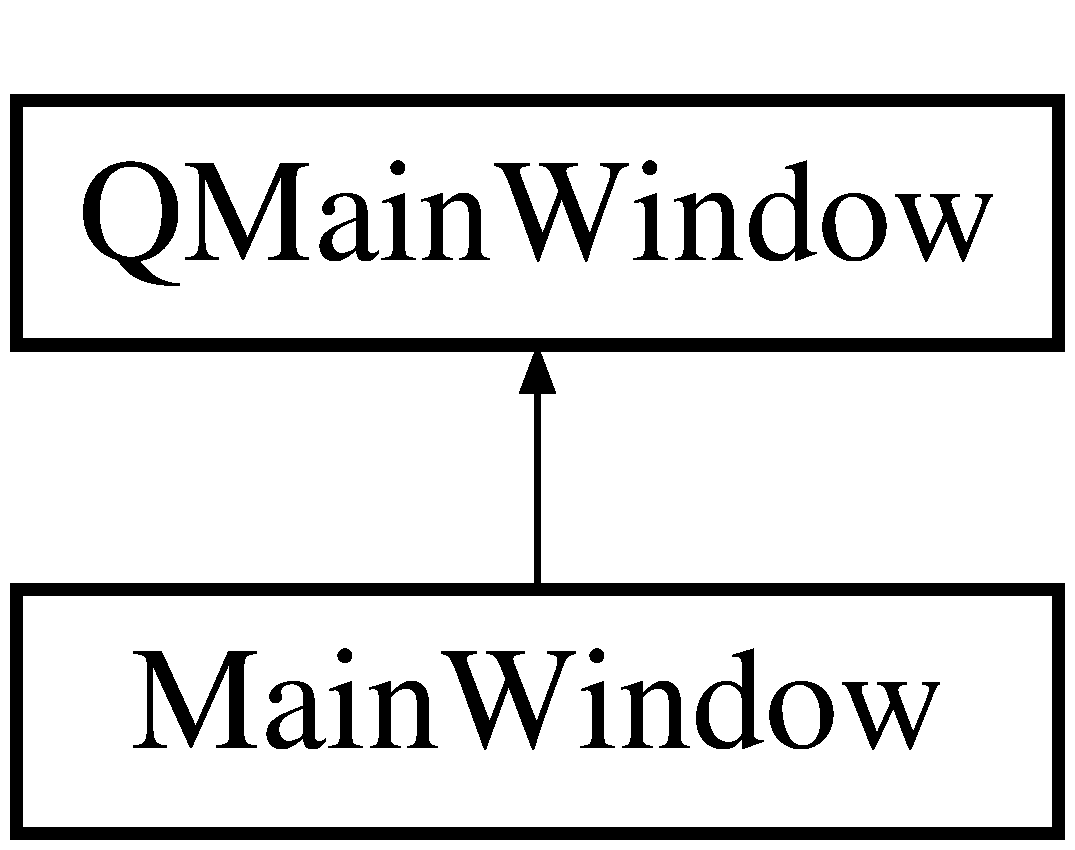
\includegraphics[height=2.000000cm]{classMainWindow}
\end{center}
\end{figure}
\subsection*{Signals}
\begin{DoxyCompactItemize}
\item 
\hypertarget{classMainWindow_a9707f0cc964479508e125742fcf94f82}{void {\bfseries Quit\-Main\-Window} ()}\label{classMainWindow_a9707f0cc964479508e125742fcf94f82}

\end{DoxyCompactItemize}
\subsection*{Public Member Functions}
\begin{DoxyCompactItemize}
\item 
\hypertarget{classMainWindow_a8b244be8b7b7db1b08de2a2acb9409db}{{\bfseries Main\-Window} (Q\-Widget $\ast$parent=0)}\label{classMainWindow_a8b244be8b7b7db1b08de2a2acb9409db}

\item 
\hypertarget{classMainWindow_a7d24542d1fbdffd9537ceb421353c860}{{\bfseries Main\-Window} (Q\-Translator $\ast$translator, Q\-Widget $\ast$parent=0)}\label{classMainWindow_a7d24542d1fbdffd9537ceb421353c860}

\item 
\hypertarget{classMainWindow_aaedb921530e29c02b7746ae62ce62ddf}{\hyperlink{classGameView}{Game\-View} $\ast$ {\bfseries Get\-Game\-View} () const }\label{classMainWindow_aaedb921530e29c02b7746ae62ce62ddf}

\item 
\hypertarget{classMainWindow_a8c6fb0a68de0e1af14efba33f90d6eae}{void \hyperlink{classMainWindow_a8c6fb0a68de0e1af14efba33f90d6eae}{Show\-Game\-View} ()}\label{classMainWindow_a8c6fb0a68de0e1af14efba33f90d6eae}

\begin{DoxyCompactList}\small\item\em Show\-Game\-View. \end{DoxyCompactList}\item 
\hypertarget{classMainWindow_ad1f9c6b77e288f15777f03d53244a9c2}{void \hyperlink{classMainWindow_ad1f9c6b77e288f15777f03d53244a9c2}{Show\-Pause\-Menu} ()}\label{classMainWindow_ad1f9c6b77e288f15777f03d53244a9c2}

\begin{DoxyCompactList}\small\item\em Show\-Pause\-Menu. \end{DoxyCompactList}\item 
\hypertarget{classMainWindow_a9069444f88de1d1b55eadd1eb7a65f2a}{void {\bfseries Change\-Language} ()}\label{classMainWindow_a9069444f88de1d1b55eadd1eb7a65f2a}

\item 
\hypertarget{classMainWindow_ac7c881667b4ba4986b5a0030452ee3f0}{void {\bfseries change\-Event} (Q\-Event $\ast$event)}\label{classMainWindow_ac7c881667b4ba4986b5a0030452ee3f0}

\item 
\hypertarget{classMainWindow_ac63b1d94f5cb0ad40b6ce651c8786b18}{void {\bfseries show\-New\-Session\-Menu} ()}\label{classMainWindow_ac63b1d94f5cb0ad40b6ce651c8786b18}

\item 
\hypertarget{classMainWindow_a63f8a7b5189797e75f175da1949a1e76}{void {\bfseries show\-Start\-Menu} ()}\label{classMainWindow_a63f8a7b5189797e75f175da1949a1e76}

\item 
\hypertarget{classMainWindow_a7d14a8a706385f2596c38b3e7c8d8fb0}{void {\bfseries show\-Highscore\-Menu} ()}\label{classMainWindow_a7d14a8a706385f2596c38b3e7c8d8fb0}

\item 
\hypertarget{classMainWindow_a4195422fe1346c1aa9c640715dfe73cb}{void {\bfseries start\-New\-Game} ()}\label{classMainWindow_a4195422fe1346c1aa9c640715dfe73cb}

\end{DoxyCompactItemize}


\subsection{Detailed Description}
The \hyperlink{classMainWindow}{Main\-Window} class. 

The content of the Sogo-\/\-App.

\begin{DoxyAuthor}{Author}
Nils Brandt 

Alexander Luedke
\end{DoxyAuthor}
\begin{DoxyDate}{Date}
08. August 2016
\end{DoxyDate}
\begin{DoxyVersion}{Version}
1.\-0 Add Documentation 
\end{DoxyVersion}

\hypertarget{classNewSessionMenu}{\section{New\-Session\-Menu Class Reference}
\label{classNewSessionMenu}\index{New\-Session\-Menu@{New\-Session\-Menu}}
}
Inheritance diagram for New\-Session\-Menu\-:\begin{figure}[H]
\begin{center}
\leavevmode
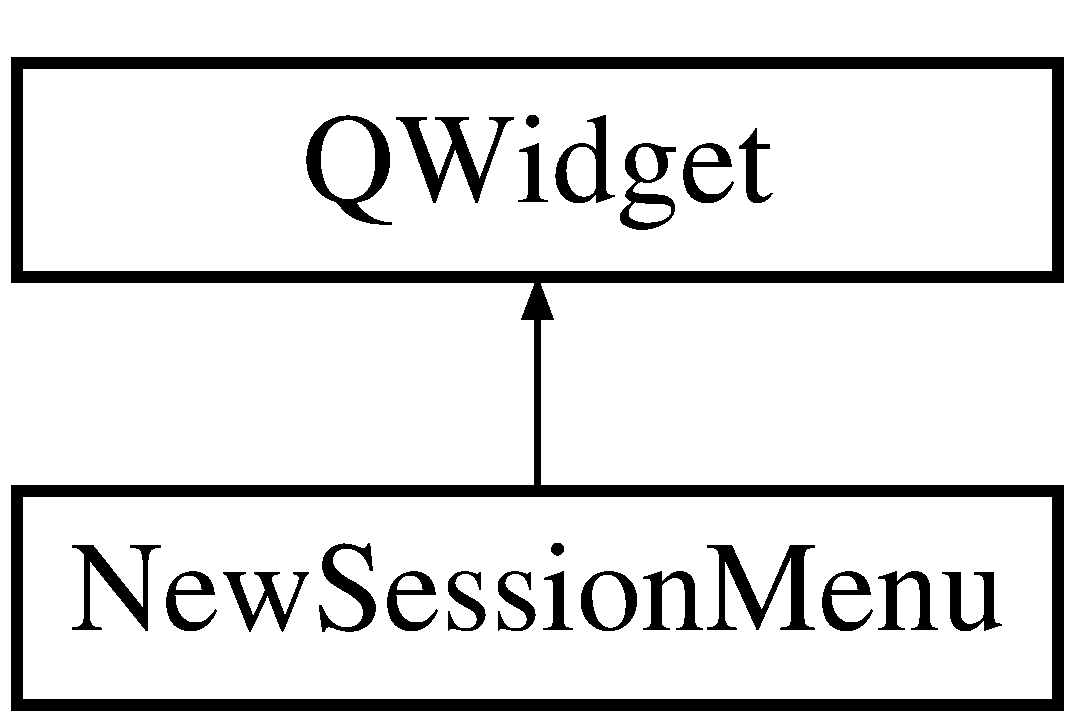
\includegraphics[height=2.000000cm]{classNewSessionMenu}
\end{center}
\end{figure}
\subsection*{Signals}
\begin{DoxyCompactItemize}
\item 
\hypertarget{classNewSessionMenu_aec46b3d790d583bd0c0fb35a7cc89d58}{void {\bfseries show\-Start\-Menu} ()}\label{classNewSessionMenu_aec46b3d790d583bd0c0fb35a7cc89d58}

\item 
\hypertarget{classNewSessionMenu_add9c9c91b8f92fde390187463b1f40ba}{void {\bfseries create\-Game\-Data} (\hyperlink{classGameData}{Game\-Data} game\-Data)}\label{classNewSessionMenu_add9c9c91b8f92fde390187463b1f40ba}

\item 
\hypertarget{classNewSessionMenu_afa1a5423cfcb5af562e30d1f66040ce5}{void {\bfseries start\-Game} ()}\label{classNewSessionMenu_afa1a5423cfcb5af562e30d1f66040ce5}

\end{DoxyCompactItemize}
\subsection*{Public Member Functions}
\begin{DoxyCompactItemize}
\item 
\hypertarget{classNewSessionMenu_a4742167534b8efad3a8163ac3d243b1b}{void {\bfseries set\-Playfield} ()}\label{classNewSessionMenu_a4742167534b8efad3a8163ac3d243b1b}

\item 
\hypertarget{classNewSessionMenu_afae85196d39cd5b68e445659faf3f901}{void {\bfseries set\-Mode} ()}\label{classNewSessionMenu_afae85196d39cd5b68e445659faf3f901}

\item 
\hypertarget{classNewSessionMenu_abe4916445e5ce3edfe78adb89533f230}{void {\bfseries change\-Event} (Q\-Event $\ast$event)}\label{classNewSessionMenu_abe4916445e5ce3edfe78adb89533f230}

\item 
\hypertarget{classNewSessionMenu_ae1038e3894d95dd28e7e9bde54fdc5eb}{{\bfseries New\-Session\-Menu} (Q\-Widget $\ast$parent=0)}\label{classNewSessionMenu_ae1038e3894d95dd28e7e9bde54fdc5eb}

\item 
\hypertarget{classNewSessionMenu_a3a5d3b6d5f3039c7ff2e4933bde10a70}{void {\bfseries merge\-Game\-Data} ()}\label{classNewSessionMenu_a3a5d3b6d5f3039c7ff2e4933bde10a70}

\item 
\hypertarget{classNewSessionMenu_a51512ad474fdb0eb6b880d17a5ce4d11}{void {\bfseries check\-Playfield\-Size} ()}\label{classNewSessionMenu_a51512ad474fdb0eb6b880d17a5ce4d11}

\item 
\hypertarget{classNewSessionMenu_ac13a0674e7492b42279b60e8b73fb561}{void {\bfseries set\-Player} ()}\label{classNewSessionMenu_ac13a0674e7492b42279b60e8b73fb561}

\item 
\hypertarget{classNewSessionMenu_a0985b4cc0908c662788f68dd55b38472}{void {\bfseries check\-Skill} ()}\label{classNewSessionMenu_a0985b4cc0908c662788f68dd55b38472}

\item 
\hypertarget{classNewSessionMenu_a30076610330be4a709eb9c72b3ec9c30}{void {\bfseries set\-Game\-Enviorment} ()}\label{classNewSessionMenu_a30076610330be4a709eb9c72b3ec9c30}

\end{DoxyCompactItemize}
\subsection*{Public Attributes}
\begin{DoxyCompactItemize}
\item 
\hypertarget{classNewSessionMenu_a1e5fc5bfe12c63b0f99df1dc3ffec0ba}{\hyperlink{classGameData}{Game\-Data} $\ast$ {\bfseries m\-\_\-game\-Data}}\label{classNewSessionMenu_a1e5fc5bfe12c63b0f99df1dc3ffec0ba}

\end{DoxyCompactItemize}


The documentation for this class was generated from the following files\-:\begin{DoxyCompactItemize}
\item 
/home/alex/source\-Code/git\-Project/beleg\-Arbeit\-E\-M\-M\-S/project\-Sogo/include/gui/New\-Session\-Menu.\-h\item 
/home/alex/source\-Code/git\-Project/beleg\-Arbeit\-E\-M\-M\-S/project\-Sogo/build-\/sogo\-App-\/\-Desktop\-\_\-\-Qt\-\_\-5\-\_\-6\-\_\-0\-\_\-\-G\-C\-C\-\_\-64bit-\/\-Debug/moc\-\_\-\-New\-Session\-Menu.\-cpp\item 
/home/alex/source\-Code/git\-Project/beleg\-Arbeit\-E\-M\-M\-S/project\-Sogo/src/gui/New\-Session\-Menu.\-cpp\end{DoxyCompactItemize}

\hypertarget{classPauseMenu}{\section{Pause\-Menu Class Reference}
\label{classPauseMenu}\index{Pause\-Menu@{Pause\-Menu}}
}


The \hyperlink{classPauseMenu}{Pause\-Menu} class.  




{\ttfamily \#include $<$Pause\-Menu.\-h$>$}

Inheritance diagram for Pause\-Menu\-:\begin{figure}[H]
\begin{center}
\leavevmode
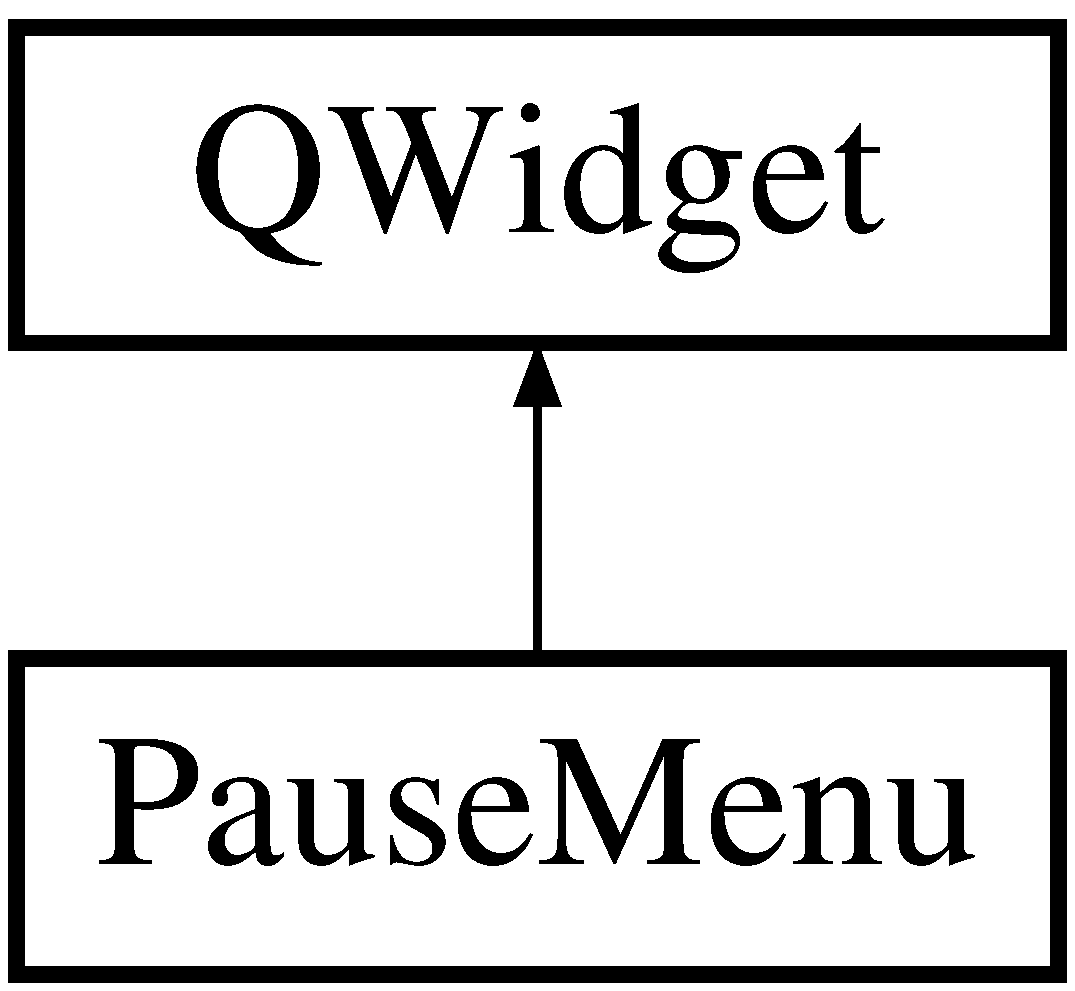
\includegraphics[height=2.000000cm]{classPauseMenu}
\end{center}
\end{figure}
\subsection*{Signals}
\begin{DoxyCompactItemize}
\item 
\hypertarget{classPauseMenu_ac24806b40fa10843a42f3d3ba96e3e6c}{void {\bfseries Resume\-Button\-Pressed} ()}\label{classPauseMenu_ac24806b40fa10843a42f3d3ba96e3e6c}

\item 
\hypertarget{classPauseMenu_a1525fb2d41bade59de33cad48d23b9d8}{void {\bfseries Save\-Button\-Pressed} ()}\label{classPauseMenu_a1525fb2d41bade59de33cad48d23b9d8}

\item 
\hypertarget{classPauseMenu_af1e7daf3f16ddca8633d9ee393f33dbb}{void {\bfseries Quit\-Game\-Button\-Pressed} ()}\label{classPauseMenu_af1e7daf3f16ddca8633d9ee393f33dbb}

\end{DoxyCompactItemize}
\subsection*{Public Member Functions}
\begin{DoxyCompactItemize}
\item 
\hypertarget{classPauseMenu_a7e37f17609a107981090585aad89a1ec}{{\bfseries Pause\-Menu} (Q\-Widget $\ast$parent=0)}\label{classPauseMenu_a7e37f17609a107981090585aad89a1ec}

\item 
\hypertarget{classPauseMenu_a7ae2f7ecbb859e6370d474db4d086892}{void {\bfseries change\-Event} (Q\-Event $\ast$event)}\label{classPauseMenu_a7ae2f7ecbb859e6370d474db4d086892}

\end{DoxyCompactItemize}


\subsection{Detailed Description}
The \hyperlink{classPauseMenu}{Pause\-Menu} class. 

To interruppt the game.

\begin{DoxyAuthor}{Author}
Nils Brandt 

Alexander Luedke
\end{DoxyAuthor}
\begin{DoxyDate}{Date}
08. August 2016
\end{DoxyDate}
\begin{DoxyVersion}{Version}
1.\-0 Add Documentation 
\end{DoxyVersion}

\hypertarget{classPlayer}{\section{Player Class Reference}
\label{classPlayer}\index{Player@{Player}}
}


The \hyperlink{classPlayer}{Player} class.  




{\ttfamily \#include $<$Player.\-h$>$}

\subsection*{Public Types}
\begin{DoxyCompactItemize}
\item 
enum \hyperlink{classPlayer_a97dc3c423902370176605121e8f68415}{Player\-Type} \{ {\bfseries H\-U\-M\-A\-N}, 
{\bfseries A\-I}
 \}
\begin{DoxyCompactList}\small\item\em The Player\-Type enum defines which type the player can be of who is playing the game. \end{DoxyCompactList}\end{DoxyCompactItemize}
\subsection*{Public Member Functions}
\begin{DoxyCompactItemize}
\item 
\hypertarget{classPlayer_affe0cc3cb714f6deb4e62f0c0d3f1fd8}{\hyperlink{classPlayer_affe0cc3cb714f6deb4e62f0c0d3f1fd8}{Player} ()}\label{classPlayer_affe0cc3cb714f6deb4e62f0c0d3f1fd8}

\begin{DoxyCompactList}\small\item\em \hyperlink{classPlayer}{Player}. \end{DoxyCompactList}\item 
\hyperlink{classPlayer_a66f0cbcaa9de5f81fcbb4ee72d0f110e}{Player} (\hyperlink{classPlayer_a97dc3c423902370176605121e8f68415}{Player\-Type} type, std\-::string name, \hyperlink{classPlayingField_ac6df152a3f820aa04a00ab4df4a9d265}{Playing\-Field\-::\-Occupation\-State} color, unsigned int skill=0)
\begin{DoxyCompactList}\small\item\em \hyperlink{classPlayer}{Player}. \end{DoxyCompactList}\item 
\hyperlink{classPlayer_a6d2881f060b07eb48077cad6044fcd8f}{Player} (const \hyperlink{classPlayer}{Player} \&src)
\begin{DoxyCompactList}\small\item\em \hyperlink{classPlayer}{Player}. \end{DoxyCompactList}\item 
\hyperlink{classPlayer_a97dc3c423902370176605121e8f68415}{Player\-Type} \hyperlink{classPlayer_adbb81c3cffe824c9ed8e18f1f635a1a3}{Get\-Type} () const 
\begin{DoxyCompactList}\small\item\em Get\-Type. \end{DoxyCompactList}\item 
std\-::string \hyperlink{classPlayer_aa5030908379dbc95594e4a9856758fef}{Get\-Name} () const 
\begin{DoxyCompactList}\small\item\em Get\-Name. \end{DoxyCompactList}\item 
\hyperlink{classPlayingField_ac6df152a3f820aa04a00ab4df4a9d265}{Playing\-Field\-::\-Occupation\-State} \hyperlink{classPlayer_a49f420e5204c895b9a94f07f6aaf639f}{Get\-Color} () const 
\begin{DoxyCompactList}\small\item\em Get\-Color. \end{DoxyCompactList}\item 
void \hyperlink{classPlayer_ac6727206628d233b9094c8e80f777c1d}{Set\-Name} (std\-::string name)
\begin{DoxyCompactList}\small\item\em Set\-Name. \end{DoxyCompactList}\item 
int \hyperlink{classPlayer_a9d8cedd46573b958fe6febbf89d07322}{Get\-Skill} () const 
\begin{DoxyCompactList}\small\item\em Get\-Skill. \end{DoxyCompactList}\item 
void \hyperlink{classPlayer_a432304cacd50b399038ea787d65464cc}{Set\-Skill} (int skill)
\begin{DoxyCompactList}\small\item\em Set\-Skill. \end{DoxyCompactList}\end{DoxyCompactItemize}
\subsection*{Static Public Member Functions}
\begin{DoxyCompactItemize}
\item 
\hypertarget{classPlayer_a4847e9d725d82c06e3cad28a12deadb4}{static string {\bfseries Serialize} (const \hyperlink{classPlayer}{Player} p)}\label{classPlayer_a4847e9d725d82c06e3cad28a12deadb4}

\item 
\hypertarget{classPlayer_a5db86c30afa559aa2cf7a95e661b262c}{static \hyperlink{classPlayer}{Player} $\ast$ {\bfseries Deserialize} (std\-::string str)  throw (\-Deserialization\-Exception)}\label{classPlayer_a5db86c30afa559aa2cf7a95e661b262c}

\end{DoxyCompactItemize}


\subsection{Detailed Description}
The \hyperlink{classPlayer}{Player} class. 

Defines a \hyperlink{classPlayer}{Player} that is defined by the type, which the player belongs to ( human or ai player ) a name a Color ( Currently Occupationstate ) skill ( currently only effectively used by ai)

\begin{DoxyAuthor}{Author}
Nils Brandt 

Alexander Luedke
\end{DoxyAuthor}
\begin{DoxyDate}{Date}
08. August 2016
\end{DoxyDate}
\begin{DoxyVersion}{Version}
1.\-0 Add Documentation 
\end{DoxyVersion}


\subsection{Constructor \& Destructor Documentation}
\hypertarget{classPlayer_a66f0cbcaa9de5f81fcbb4ee72d0f110e}{\index{Player@{Player}!Player@{Player}}
\index{Player@{Player}!Player@{Player}}
\subsubsection[{Player}]{\setlength{\rightskip}{0pt plus 5cm}Player\-::\-Player (
\begin{DoxyParamCaption}
\item[{{\bf Player\-Type}}]{type, }
\item[{std\-::string}]{name, }
\item[{{\bf Playing\-Field\-::\-Occupation\-State}}]{color, }
\item[{unsigned int}]{skill = {\ttfamily 0}}
\end{DoxyParamCaption}
)}}\label{classPlayer_a66f0cbcaa9de5f81fcbb4ee72d0f110e}


\hyperlink{classPlayer}{Player}. 


\begin{DoxyParams}{Parameters}
{\em type} & \\
\hline
{\em name} & \\
\hline
{\em color} & \\
\hline
{\em skill} & \\
\hline
\end{DoxyParams}
\hypertarget{classPlayer_a6d2881f060b07eb48077cad6044fcd8f}{\index{Player@{Player}!Player@{Player}}
\index{Player@{Player}!Player@{Player}}
\subsubsection[{Player}]{\setlength{\rightskip}{0pt plus 5cm}Player\-::\-Player (
\begin{DoxyParamCaption}
\item[{const {\bf Player} \&}]{src}
\end{DoxyParamCaption}
)}}\label{classPlayer_a6d2881f060b07eb48077cad6044fcd8f}


\hyperlink{classPlayer}{Player}. 


\begin{DoxyParams}{Parameters}
{\em src} & \\
\hline
\end{DoxyParams}


\subsection{Member Function Documentation}
\hypertarget{classPlayer_a49f420e5204c895b9a94f07f6aaf639f}{\index{Player@{Player}!Get\-Color@{Get\-Color}}
\index{Get\-Color@{Get\-Color}!Player@{Player}}
\subsubsection[{Get\-Color}]{\setlength{\rightskip}{0pt plus 5cm}{\bf Playing\-Field\-::\-Occupation\-State} Player\-::\-Get\-Color (
\begin{DoxyParamCaption}
{}
\end{DoxyParamCaption}
) const}}\label{classPlayer_a49f420e5204c895b9a94f07f6aaf639f}


Get\-Color. 

\begin{DoxyReturn}{Returns}

\end{DoxyReturn}
\hypertarget{classPlayer_aa5030908379dbc95594e4a9856758fef}{\index{Player@{Player}!Get\-Name@{Get\-Name}}
\index{Get\-Name@{Get\-Name}!Player@{Player}}
\subsubsection[{Get\-Name}]{\setlength{\rightskip}{0pt plus 5cm}std\-::string Player\-::\-Get\-Name (
\begin{DoxyParamCaption}
{}
\end{DoxyParamCaption}
) const}}\label{classPlayer_aa5030908379dbc95594e4a9856758fef}


Get\-Name. 

\begin{DoxyReturn}{Returns}

\end{DoxyReturn}
\hypertarget{classPlayer_a9d8cedd46573b958fe6febbf89d07322}{\index{Player@{Player}!Get\-Skill@{Get\-Skill}}
\index{Get\-Skill@{Get\-Skill}!Player@{Player}}
\subsubsection[{Get\-Skill}]{\setlength{\rightskip}{0pt plus 5cm}int Player\-::\-Get\-Skill (
\begin{DoxyParamCaption}
{}
\end{DoxyParamCaption}
) const}}\label{classPlayer_a9d8cedd46573b958fe6febbf89d07322}


Get\-Skill. 

\begin{DoxyReturn}{Returns}

\end{DoxyReturn}
\hypertarget{classPlayer_adbb81c3cffe824c9ed8e18f1f635a1a3}{\index{Player@{Player}!Get\-Type@{Get\-Type}}
\index{Get\-Type@{Get\-Type}!Player@{Player}}
\subsubsection[{Get\-Type}]{\setlength{\rightskip}{0pt plus 5cm}{\bf Player\-::\-Player\-Type} Player\-::\-Get\-Type (
\begin{DoxyParamCaption}
{}
\end{DoxyParamCaption}
) const}}\label{classPlayer_adbb81c3cffe824c9ed8e18f1f635a1a3}


Get\-Type. 

\begin{DoxyReturn}{Returns}

\end{DoxyReturn}
\hypertarget{classPlayer_ac6727206628d233b9094c8e80f777c1d}{\index{Player@{Player}!Set\-Name@{Set\-Name}}
\index{Set\-Name@{Set\-Name}!Player@{Player}}
\subsubsection[{Set\-Name}]{\setlength{\rightskip}{0pt plus 5cm}void Player\-::\-Set\-Name (
\begin{DoxyParamCaption}
\item[{std\-::string}]{name}
\end{DoxyParamCaption}
)}}\label{classPlayer_ac6727206628d233b9094c8e80f777c1d}


Set\-Name. 


\begin{DoxyParams}{Parameters}
{\em name} & \\
\hline
\end{DoxyParams}
\hypertarget{classPlayer_a432304cacd50b399038ea787d65464cc}{\index{Player@{Player}!Set\-Skill@{Set\-Skill}}
\index{Set\-Skill@{Set\-Skill}!Player@{Player}}
\subsubsection[{Set\-Skill}]{\setlength{\rightskip}{0pt plus 5cm}void Player\-::\-Set\-Skill (
\begin{DoxyParamCaption}
\item[{int}]{skill}
\end{DoxyParamCaption}
)}}\label{classPlayer_a432304cacd50b399038ea787d65464cc}


Set\-Skill. 


\begin{DoxyParams}{Parameters}
{\em skill} & \\
\hline
\end{DoxyParams}

\hypertarget{classPlayerInput}{\section{Player\-Input Class Reference}
\label{classPlayerInput}\index{Player\-Input@{Player\-Input}}
}


The \hyperlink{classPlayerInput}{Player\-Input} class.  




{\ttfamily \#include $<$Player\-Input.\-h$>$}

Inheritance diagram for Player\-Input\-:\begin{figure}[H]
\begin{center}
\leavevmode
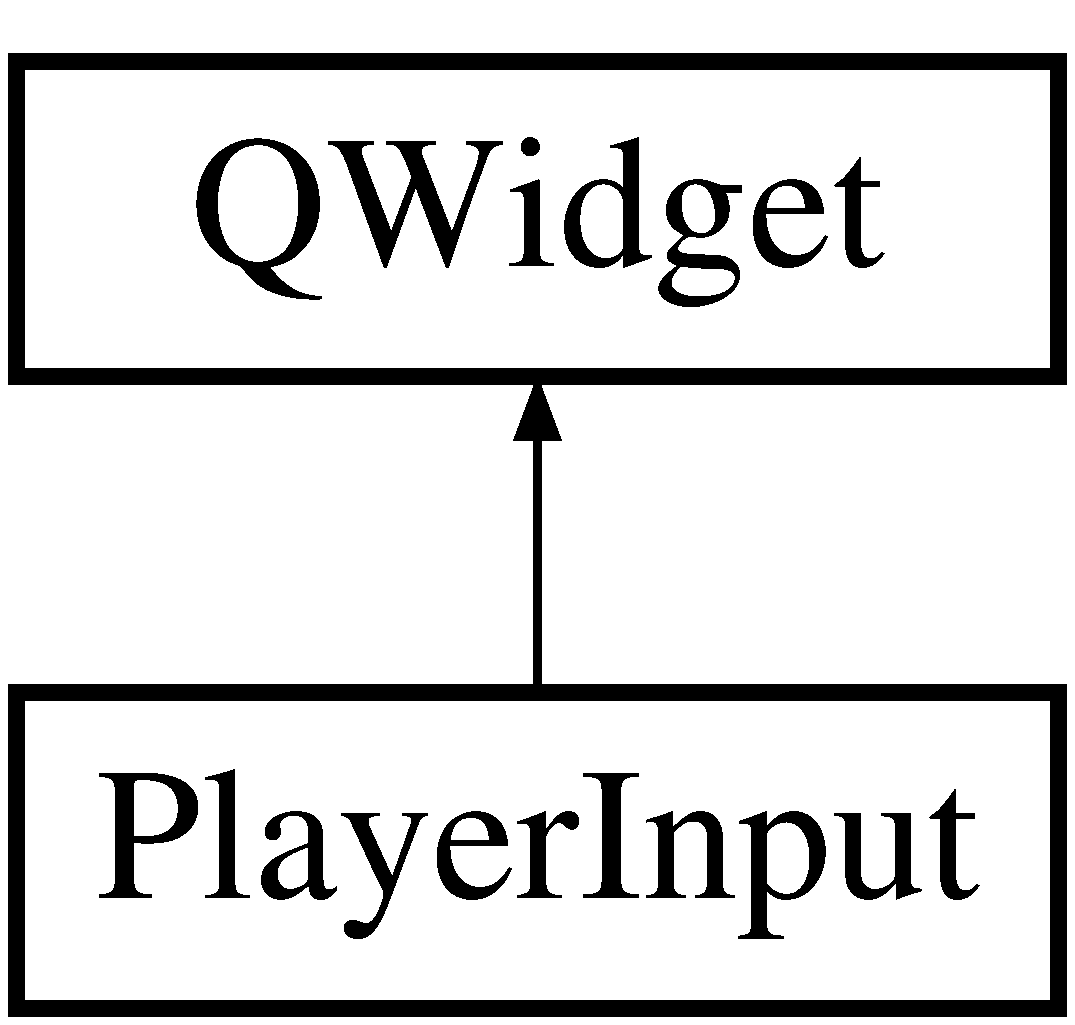
\includegraphics[height=2.000000cm]{classPlayerInput}
\end{center}
\end{figure}
\subsection*{Signals}
\begin{DoxyCompactItemize}
\item 
void \hyperlink{classPlayerInput_aab7de51daaa958792ffaae64e41f43e6}{Input\-Confirmed} (\hyperlink{structVector2}{Vector2} pos)
\begin{DoxyCompactList}\small\item\em To confirm the playerinput. \end{DoxyCompactList}\end{DoxyCompactItemize}
\subsection*{Public Member Functions}
\begin{DoxyCompactItemize}
\item 
\hypertarget{classPlayerInput_a41adeb104eebbd46404b0a29203441c5}{{\bfseries Player\-Input} (\hyperlink{classGameManager}{Game\-Manager} $\ast$game\-Manager, Q\-Widget $\ast$parent=0)}\label{classPlayerInput_a41adeb104eebbd46404b0a29203441c5}

\item 
\hypertarget{classPlayerInput_ab8abc1017f5b0e8589fbf1b8b550eba4}{void {\bfseries change\-Event} (Q\-Event $\ast$event)}\label{classPlayerInput_ab8abc1017f5b0e8589fbf1b8b550eba4}

\item 
\hypertarget{classPlayerInput_a2135e14f7e216f1f78ab63212230aa03}{void {\bfseries Apply\-Player\-Change} ()}\label{classPlayerInput_a2135e14f7e216f1f78ab63212230aa03}

\end{DoxyCompactItemize}


\subsection{Detailed Description}
The \hyperlink{classPlayerInput}{Player\-Input} class. 

\begin{DoxyAuthor}{Author}
Nils Brandt 

Alexander Luedke
\end{DoxyAuthor}
\begin{DoxyDate}{Date}
08. August 2016
\end{DoxyDate}
\begin{DoxyVersion}{Version}
1.\-0 Add Documentation 
\end{DoxyVersion}


\subsection{Member Function Documentation}
\hypertarget{classPlayerInput_aab7de51daaa958792ffaae64e41f43e6}{\index{Player\-Input@{Player\-Input}!Input\-Confirmed@{Input\-Confirmed}}
\index{Input\-Confirmed@{Input\-Confirmed}!PlayerInput@{Player\-Input}}
\subsubsection[{Input\-Confirmed}]{\setlength{\rightskip}{0pt plus 5cm}void Player\-Input\-::\-Input\-Confirmed (
\begin{DoxyParamCaption}
\item[{{\bf Vector2}}]{pos}
\end{DoxyParamCaption}
)\hspace{0.3cm}{\ttfamily [signal]}}}\label{classPlayerInput_aab7de51daaa958792ffaae64e41f43e6}


To confirm the playerinput. 


\begin{DoxyParams}{Parameters}
{\em pos} & The position the player wants to set. \\
\hline
\end{DoxyParams}

\hypertarget{classPlayingField}{\section{Playing\-Field Class Reference}
\label{classPlayingField}\index{Playing\-Field@{Playing\-Field}}
}


Defines the Properties of a Playingfield.  




{\ttfamily \#include $<$Playing\-Field.\-h$>$}

\subsection*{Classes}
\begin{DoxyCompactItemize}
\item 
struct \hyperlink{structPlayingField_1_1Slot}{Slot}
\begin{DoxyCompactList}\small\item\em Defines a Gridspace in a Sogo Playingfield It contains the occupationstate of this position in the grid. \end{DoxyCompactList}\end{DoxyCompactItemize}
\subsection*{Public Types}
\begin{DoxyCompactItemize}
\item 
enum \hyperlink{classPlayingField_a6032d4d7297d628a368cde7db331d7f6}{Field\-Exeptions} \{ {\bfseries O\-C\-C\-U\-P\-I\-E\-D}, 
{\bfseries P\-O\-S\-I\-T\-I\-O\-N\-\_\-\-N\-O\-T\-\_\-\-A\-V\-A\-I\-L\-A\-B\-L\-E}, 
{\bfseries N\-O\-\_\-\-S\-P\-A\-C\-E\-\_\-\-A\-N\-Y\-M\-O\-R\-E}
 \}
\begin{DoxyCompactList}\small\item\em Is thrown when in an Error in Playingfield O\-C\-C\-U\-P\-I\-E\-D when already occupied by other player P\-O\-S\-I\-T\-I\-O\-N\-\_\-\-N\-O\-T\-\_\-\-A\-V\-A\-I\-L\-A\-B\-L\-E when position is not valid for occupation under current circumstances. \end{DoxyCompactList}\item 
enum \hyperlink{classPlayingField_ac6df152a3f820aa04a00ab4df4a9d265}{Occupation\-State} \{ {\bfseries N\-O\-N\-E}, 
{\bfseries R\-E\-D}, 
{\bfseries B\-L\-U\-E}
 \}
\begin{DoxyCompactList}\small\item\em Defines the States a slot can be in. \end{DoxyCompactList}\end{DoxyCompactItemize}
\subsection*{Public Member Functions}
\begin{DoxyCompactItemize}
\item 
\hyperlink{classPlayingField_a9cd7d0540bff01b5b83ca9bdf8dfd5d6}{Playing\-Field} (int field\-Size=4)
\begin{DoxyCompactList}\small\item\em constructor generates a Playingfield with (fieldsize x fieldsize x fieldsize) \end{DoxyCompactList}\item 
\hypertarget{classPlayingField_a4715051a7ba2b0495b3b56d357563432}{\hyperlink{classPlayingField_a4715051a7ba2b0495b3b56d357563432}{Playing\-Field} (const \hyperlink{classPlayingField}{Playing\-Field} \&field)}\label{classPlayingField_a4715051a7ba2b0495b3b56d357563432}

\begin{DoxyCompactList}\small\item\em Copy constructor. \end{DoxyCompactList}\item 
\hypertarget{classPlayingField_a7bc092c6433f18e7a07835608e8a4449}{\hyperlink{classPlayingField_a7bc092c6433f18e7a07835608e8a4449}{$\sim$\-Playing\-Field} ()}\label{classPlayingField_a7bc092c6433f18e7a07835608e8a4449}

\begin{DoxyCompactList}\small\item\em Destructor clears the field. \end{DoxyCompactList}\item 
\hyperlink{structPlayingField_1_1Slot}{Slot} $\ast$ \hyperlink{classPlayingField_a01b5105b49ec72e094411d216df27ffa}{Get\-Slot} (int x, int y, int z) const   throw (out\-\_\-of\-\_\-range)
\begin{DoxyCompactList}\small\item\em Returns the slot at pos.\-x (horizontally) pos.\-y (Vertically) pos.\-z (\char`\"{}forwardly\char`\"{}) \end{DoxyCompactList}\item 
int \hyperlink{classPlayingField_abfbecf0f8ba91c9c1167da359e7463dc}{Get\-Field\-Size} () const 
\begin{DoxyCompactList}\small\item\em Getter for field\-Size. \end{DoxyCompactList}\item 
void \hyperlink{classPlayingField_a166ff0aaa90a41ce748efd9165a9d578}{Occupy\-Slot} (int x, int y, int z, \hyperlink{classPlayingField_ac6df152a3f820aa04a00ab4df4a9d265}{Occupation\-State} id)  throw (out\-\_\-of\-\_\-range, Field\-Exeptions)
\begin{DoxyCompactList}\small\item\em Sets the occupation\-State of the \hyperlink{structPlayingField_1_1Slot}{Slot} at pos(x,y,z) to id. \end{DoxyCompactList}\item 
void \hyperlink{classPlayingField_a6165557999a6cec6c1c1b71b88c2f82e}{Occupy\-Slot} (\hyperlink{structVector3}{Vector3} pos, \hyperlink{classPlayingField_ac6df152a3f820aa04a00ab4df4a9d265}{Playing\-Field\-::\-Occupation\-State} id)  throw (out\-\_\-of\-\_\-range, Field\-Exeptions)
\begin{DoxyCompactList}\small\item\em Sets the occupation\-State of the \hyperlink{structPlayingField_1_1Slot}{Slot} at pos(x,y,z) to id. \end{DoxyCompactList}\item 
\hypertarget{classPlayingField_af25e735d1d9f1c561fdf951507b2c1de}{bool {\bfseries Is\-Position\-Available} (int x, int y, int z) const }\label{classPlayingField_af25e735d1d9f1c561fdf951507b2c1de}

\end{DoxyCompactItemize}
\subsection*{Static Public Member Functions}
\begin{DoxyCompactItemize}
\item 
\hypertarget{classPlayingField_ad0b87276c478b016d1425e7d69ba4e73}{static std\-::string {\bfseries Serialize} (const \hyperlink{classPlayingField}{Playing\-Field} \&p\-F)}\label{classPlayingField_ad0b87276c478b016d1425e7d69ba4e73}

\item 
\hypertarget{classPlayingField_a4fca00ce844080c76d91d45f4937d4cc}{static \hyperlink{classPlayingField}{Playing\-Field} $\ast$ {\bfseries Deserialize} (string str)  throw (\-Deserialization\-Exception)}\label{classPlayingField_a4fca00ce844080c76d91d45f4937d4cc}

\end{DoxyCompactItemize}


\subsection{Detailed Description}
Defines the Properties of a Playingfield. 

Which is a 3 dimensional Grid Containing Slots Slots can be occupied by players

\begin{DoxyAuthor}{Author}
Nils Brandt 

Alexander Luedke
\end{DoxyAuthor}
\begin{DoxyDate}{Date}
08. August 2016
\end{DoxyDate}
\begin{DoxyVersion}{Version}
1.\-0 Add Documentation 
\end{DoxyVersion}


\subsection{Constructor \& Destructor Documentation}
\hypertarget{classPlayingField_a9cd7d0540bff01b5b83ca9bdf8dfd5d6}{\index{Playing\-Field@{Playing\-Field}!Playing\-Field@{Playing\-Field}}
\index{Playing\-Field@{Playing\-Field}!PlayingField@{Playing\-Field}}
\subsubsection[{Playing\-Field}]{\setlength{\rightskip}{0pt plus 5cm}Playing\-Field\-::\-Playing\-Field (
\begin{DoxyParamCaption}
\item[{int}]{field\-Size = {\ttfamily 4}}
\end{DoxyParamCaption}
)}}\label{classPlayingField_a9cd7d0540bff01b5b83ca9bdf8dfd5d6}


constructor generates a Playingfield with (fieldsize x fieldsize x fieldsize) 


\begin{DoxyParams}{Parameters}
{\em field\-Size} & (default value = 4) \\
\hline
\end{DoxyParams}


\subsection{Member Function Documentation}
\hypertarget{classPlayingField_abfbecf0f8ba91c9c1167da359e7463dc}{\index{Playing\-Field@{Playing\-Field}!Get\-Field\-Size@{Get\-Field\-Size}}
\index{Get\-Field\-Size@{Get\-Field\-Size}!PlayingField@{Playing\-Field}}
\subsubsection[{Get\-Field\-Size}]{\setlength{\rightskip}{0pt plus 5cm}int Playing\-Field\-::\-Get\-Field\-Size (
\begin{DoxyParamCaption}
{}
\end{DoxyParamCaption}
) const}}\label{classPlayingField_abfbecf0f8ba91c9c1167da359e7463dc}


Getter for field\-Size. 

\begin{DoxyReturn}{Returns}
returns the fieldsize 
\end{DoxyReturn}
\hypertarget{classPlayingField_a01b5105b49ec72e094411d216df27ffa}{\index{Playing\-Field@{Playing\-Field}!Get\-Slot@{Get\-Slot}}
\index{Get\-Slot@{Get\-Slot}!PlayingField@{Playing\-Field}}
\subsubsection[{Get\-Slot}]{\setlength{\rightskip}{0pt plus 5cm}{\bf Playing\-Field\-::\-Slot} $\ast$ Playing\-Field\-::\-Get\-Slot (
\begin{DoxyParamCaption}
\item[{int}]{x, }
\item[{int}]{y, }
\item[{int}]{z}
\end{DoxyParamCaption}
) const throw  out\-\_\-of\-\_\-range) }}\label{classPlayingField_a01b5105b49ec72e094411d216df27ffa}


Returns the slot at pos.\-x (horizontally) pos.\-y (Vertically) pos.\-z (\char`\"{}forwardly\char`\"{}) 


\begin{DoxyExceptions}{Exceptions}
{\em out\-\_\-of\-\_\-range} & if value is higher than fieldsize \\
\hline
\end{DoxyExceptions}
\hypertarget{classPlayingField_a166ff0aaa90a41ce748efd9165a9d578}{\index{Playing\-Field@{Playing\-Field}!Occupy\-Slot@{Occupy\-Slot}}
\index{Occupy\-Slot@{Occupy\-Slot}!PlayingField@{Playing\-Field}}
\subsubsection[{Occupy\-Slot}]{\setlength{\rightskip}{0pt plus 5cm}void Playing\-Field\-::\-Occupy\-Slot (
\begin{DoxyParamCaption}
\item[{int}]{x, }
\item[{int}]{y, }
\item[{int}]{z, }
\item[{{\bf Playing\-Field\-::\-Occupation\-State}}]{id}
\end{DoxyParamCaption}
) throw  out\-\_\-of\-\_\-range, {\bf Field\-Exeptions}) }}\label{classPlayingField_a166ff0aaa90a41ce748efd9165a9d578}


Sets the occupation\-State of the \hyperlink{structPlayingField_1_1Slot}{Slot} at pos(x,y,z) to id. 


\begin{DoxyParams}{Parameters}
{\em x} & horizontal value \\
\hline
{\em y} & depth value \\
\hline
{\em z} & vertical value \\
\hline
{\em id} & occupationstate for assignment \\
\hline
\end{DoxyParams}

\begin{DoxyExceptions}{Exceptions}
{\em out\-\_\-of\-\_\-range} & if value is higher than fieldsize \\
\hline
{\em Field\-Exception} & if \hyperlink{structPlayingField_1_1Slot}{Slot} is already occupied by other player \\
\hline
\end{DoxyExceptions}
\hypertarget{classPlayingField_a6165557999a6cec6c1c1b71b88c2f82e}{\index{Playing\-Field@{Playing\-Field}!Occupy\-Slot@{Occupy\-Slot}}
\index{Occupy\-Slot@{Occupy\-Slot}!PlayingField@{Playing\-Field}}
\subsubsection[{Occupy\-Slot}]{\setlength{\rightskip}{0pt plus 5cm}void Playing\-Field\-::\-Occupy\-Slot (
\begin{DoxyParamCaption}
\item[{{\bf Vector3}}]{pos, }
\item[{{\bf Playing\-Field\-::\-Occupation\-State}}]{id}
\end{DoxyParamCaption}
) throw  out\-\_\-of\-\_\-range, {\bf Field\-Exeptions}) }}\label{classPlayingField_a6165557999a6cec6c1c1b71b88c2f82e}


Sets the occupation\-State of the \hyperlink{structPlayingField_1_1Slot}{Slot} at pos(x,y,z) to id. 


\begin{DoxyParams}{Parameters}
{\em pos} & \\
\hline
{\em id} & occupationstate for assignment \\
\hline
\end{DoxyParams}

\begin{DoxyExceptions}{Exceptions}
{\em out\-\_\-of\-\_\-range} & if value is higher than fieldsize \\
\hline
{\em Field\-Exception} & if \hyperlink{structPlayingField_1_1Slot}{Slot} is already occupied by other player \\
\hline
\end{DoxyExceptions}

\hypertarget{structPlayingField_1_1Slot}{\section{Playing\-Field\-:\-:Slot Struct Reference}
\label{structPlayingField_1_1Slot}\index{Playing\-Field\-::\-Slot@{Playing\-Field\-::\-Slot}}
}


Defines a Gridspace in a Sogo Playingfield It contains the occupationstate of this position in the grid.  




{\ttfamily \#include $<$Playing\-Field.\-h$>$}

\subsection*{Public Member Functions}
\begin{DoxyCompactItemize}
\item 
\hypertarget{structPlayingField_1_1Slot_a2c572050c538c2d445597984a14df2a6}{\hyperlink{structPlayingField_1_1Slot_a2c572050c538c2d445597984a14df2a6}{Slot} ()}\label{structPlayingField_1_1Slot_a2c572050c538c2d445597984a14df2a6}

\begin{DoxyCompactList}\small\item\em Default constructor for a \hyperlink{structPlayingField_1_1Slot}{Slot} Occupation will be set to None. \end{DoxyCompactList}\item 
\hyperlink{structPlayingField_1_1Slot_ad56b4d9838d1475763c131bf310ae2d0}{Slot} (\hyperlink{classPlayingField_ac6df152a3f820aa04a00ab4df4a9d265}{Playing\-Field\-::\-Occupation\-State} occupation)
\begin{DoxyCompactList}\small\item\em constructor \end{DoxyCompactList}\end{DoxyCompactItemize}
\subsection*{Public Attributes}
\begin{DoxyCompactItemize}
\item 
\hypertarget{structPlayingField_1_1Slot_a1c4ada065c877c9dd33950a9f9eb7d4f}{\hyperlink{classPlayingField_ac6df152a3f820aa04a00ab4df4a9d265}{Playing\-Field\-::\-Occupation\-State} \hyperlink{structPlayingField_1_1Slot_a1c4ada065c877c9dd33950a9f9eb7d4f}{Occupation}}\label{structPlayingField_1_1Slot_a1c4ada065c877c9dd33950a9f9eb7d4f}

\begin{DoxyCompactList}\small\item\em The current occupation state. \end{DoxyCompactList}\end{DoxyCompactItemize}


\subsection{Detailed Description}
Defines a Gridspace in a Sogo Playingfield It contains the occupationstate of this position in the grid. 



\subsection{Constructor \& Destructor Documentation}
\hypertarget{structPlayingField_1_1Slot_ad56b4d9838d1475763c131bf310ae2d0}{\index{Playing\-Field\-::\-Slot@{Playing\-Field\-::\-Slot}!Slot@{Slot}}
\index{Slot@{Slot}!PlayingField::Slot@{Playing\-Field\-::\-Slot}}
\subsubsection[{Slot}]{\setlength{\rightskip}{0pt plus 5cm}Playing\-Field\-::\-Slot\-::\-Slot (
\begin{DoxyParamCaption}
\item[{{\bf Playing\-Field\-::\-Occupation\-State}}]{occupation}
\end{DoxyParamCaption}
)}}\label{structPlayingField_1_1Slot_ad56b4d9838d1475763c131bf310ae2d0}


constructor 



The documentation for this struct was generated from the following files\-:\begin{DoxyCompactItemize}
\item 
/home/alex/source\-Code/git\-Project/beleg\-Arbeit\-E\-M\-M\-S/project\-Sogo/include/core/Playing\-Field.\-h\item 
/home/alex/source\-Code/git\-Project/beleg\-Arbeit\-E\-M\-M\-S/project\-Sogo/src/core/Playing\-Field.\-cpp\end{DoxyCompactItemize}

\hypertarget{classStartMenu}{\section{Start\-Menu Class Reference}
\label{classStartMenu}\index{Start\-Menu@{Start\-Menu}}
}
Inheritance diagram for Start\-Menu\-:\begin{figure}[H]
\begin{center}
\leavevmode
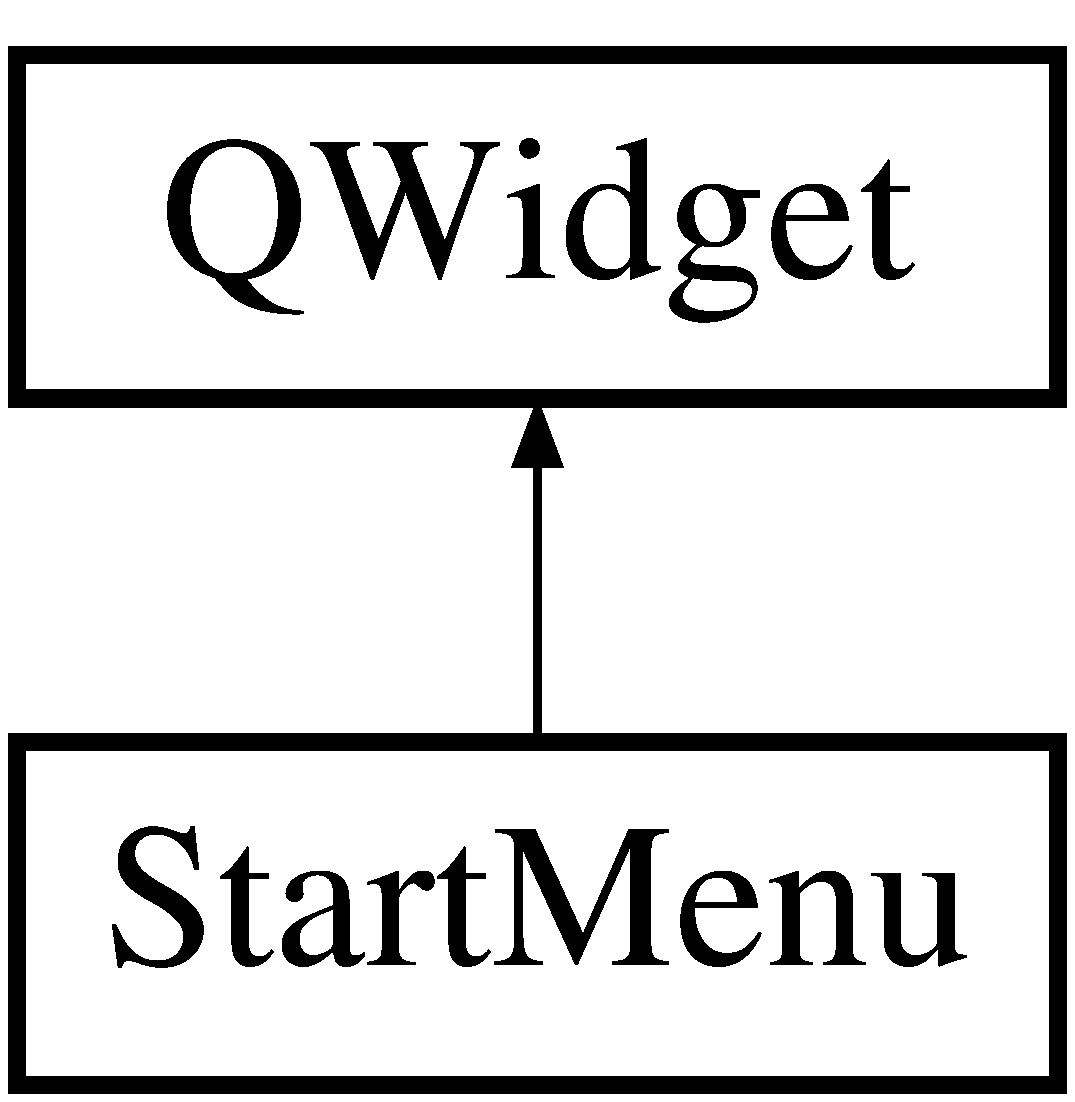
\includegraphics[height=2.000000cm]{classStartMenu}
\end{center}
\end{figure}
\subsection*{Signals}
\begin{DoxyCompactItemize}
\item 
\hypertarget{classStartMenu_a94d2da8144b5e99707ef5dc1ea588982}{void {\bfseries switch\-To\-New\-Session} ()}\label{classStartMenu_a94d2da8144b5e99707ef5dc1ea588982}

\item 
\hypertarget{classStartMenu_a95881192196673c85ad1dc12df5f9820}{void {\bfseries switch\-To\-Highscore} ()}\label{classStartMenu_a95881192196673c85ad1dc12df5f9820}

\item 
\hypertarget{classStartMenu_aff58f89652b89899b21d40f3188b516d}{void {\bfseries quit\-Game} ()}\label{classStartMenu_aff58f89652b89899b21d40f3188b516d}

\end{DoxyCompactItemize}
\subsection*{Public Member Functions}
\begin{DoxyCompactItemize}
\item 
\hypertarget{classStartMenu_a1491fb2672b951483f3cfc0594571fbb}{{\bfseries Start\-Menu} (Q\-Widget $\ast$parent=0)}\label{classStartMenu_a1491fb2672b951483f3cfc0594571fbb}

\item 
\hypertarget{classStartMenu_afc4a48db40567e80c6514b0af30d3797}{void {\bfseries change\-Event} (Q\-Event $\ast$event)}\label{classStartMenu_afc4a48db40567e80c6514b0af30d3797}

\end{DoxyCompactItemize}


The documentation for this class was generated from the following files\-:\begin{DoxyCompactItemize}
\item 
/home/alex/source\-Code/git\-Project/beleg\-Arbeit\-E\-M\-M\-S/project\-Sogo/include/gui/Start\-Menu.\-h\item 
/home/alex/source\-Code/git\-Project/beleg\-Arbeit\-E\-M\-M\-S/project\-Sogo/build-\/sogo\-App-\/\-Desktop\-\_\-\-Qt\-\_\-5\-\_\-6\-\_\-0\-\_\-\-G\-C\-C\-\_\-64bit-\/\-Debug/moc\-\_\-\-Start\-Menu.\-cpp\item 
/home/alex/source\-Code/git\-Project/beleg\-Arbeit\-E\-M\-M\-S/project\-Sogo/src/gui/Start\-Menu.\-cpp\end{DoxyCompactItemize}

\hypertarget{classSubject}{\section{Subject Class Reference}
\label{classSubject}\index{Subject@{Subject}}
}


The \hyperlink{classSubject}{Subject} class.  




{\ttfamily \#include $<$Subject.\-h$>$}

\subsection*{Public Member Functions}
\begin{DoxyCompactItemize}
\item 
\hypertarget{classSubject_ab468044832c824c6d6c2f46272655207}{\hyperlink{classSubject_ab468044832c824c6d6c2f46272655207}{Subject} ()}\label{classSubject_ab468044832c824c6d6c2f46272655207}

\begin{DoxyCompactList}\small\item\em \hyperlink{classSubject}{Subject}. \end{DoxyCompactList}\item 
\hypertarget{classSubject_ae5980067d5ec5522db5a0d78100a34be}{virtual \hyperlink{classSubject_ae5980067d5ec5522db5a0d78100a34be}{$\sim$\-Subject} ()}\label{classSubject_ae5980067d5ec5522db5a0d78100a34be}

\begin{DoxyCompactList}\small\item\em $\sim$\-Subject \end{DoxyCompactList}\item 
void \hyperlink{classSubject_ad093a7ac7fea38b82f5cc333916d4a90}{Add\-Listener} (\hyperlink{classIObserver}{I\-Observer} $\ast$obs)
\begin{DoxyCompactList}\small\item\em Add\-Listener Adds an observer to the observer list. \end{DoxyCompactList}\end{DoxyCompactItemize}
\subsection*{Protected Member Functions}
\begin{DoxyCompactItemize}
\item 
\hypertarget{classSubject_ad047f9358b9d199bca40fc5f62a26fc0}{virtual void \hyperlink{classSubject_ad047f9358b9d199bca40fc5f62a26fc0}{Notify\-All\-Observer} ()}\label{classSubject_ad047f9358b9d199bca40fc5f62a26fc0}

\begin{DoxyCompactList}\small\item\em Notify\-All\-Observer Used to Notify all observers observing this subject. \end{DoxyCompactList}\end{DoxyCompactItemize}


\subsection{Detailed Description}
The \hyperlink{classSubject}{Subject} class. 

\subsection{Member Function Documentation}
\hypertarget{classSubject_ad093a7ac7fea38b82f5cc333916d4a90}{\index{Subject@{Subject}!Add\-Listener@{Add\-Listener}}
\index{Add\-Listener@{Add\-Listener}!Subject@{Subject}}
\subsubsection[{Add\-Listener}]{\setlength{\rightskip}{0pt plus 5cm}void Subject\-::\-Add\-Listener (
\begin{DoxyParamCaption}
\item[{{\bf I\-Observer} $\ast$}]{obs}
\end{DoxyParamCaption}
)\hspace{0.3cm}{\ttfamily [inline]}}}\label{classSubject_ad093a7ac7fea38b82f5cc333916d4a90}


Add\-Listener Adds an observer to the observer list. 


\begin{DoxyParams}{Parameters}
{\em obs} & observer to be added \\
\hline
\end{DoxyParams}

\hypertarget{structVector2}{\section{Vector2 Struct Reference}
\label{structVector2}\index{Vector2@{Vector2}}
}


Defines a structures that encapsulates a position in 2\-D space.  




{\ttfamily \#include $<$Vector2.\-h$>$}

\subsection*{Public Member Functions}
\begin{DoxyCompactItemize}
\item 
\hypertarget{structVector2_a22104d1809be26a419ef1f959e3761bf}{\hyperlink{structVector2_a22104d1809be26a419ef1f959e3761bf}{Vector2} ()}\label{structVector2_a22104d1809be26a419ef1f959e3761bf}

\begin{DoxyCompactList}\small\item\em Default constructor Initializes X,Y to zero. \end{DoxyCompactList}\item 
\hypertarget{structVector2_a5292d22e63825ec0e90e1574825c9570}{{\bfseries Vector2} (const \hyperlink{structVector2}{Vector2} \&src)}\label{structVector2_a5292d22e63825ec0e90e1574825c9570}

\item 
\hyperlink{structVector2_a321cf468f0b0caa050fc802f29af48ee}{Vector2} (int x, int y)
\begin{DoxyCompactList}\small\item\em constructor \end{DoxyCompactList}\item 
\hypertarget{structVector2_a89acd25f33fbf1774fdf960e259cf170}{std\-::string {\bfseries Serialize} ()}\label{structVector2_a89acd25f33fbf1774fdf960e259cf170}

\item 
\hypertarget{structVector2_acc5476ed3ba51ab7ab9b6d49a89e8379}{void {\bfseries Deserialize} ()}\label{structVector2_acc5476ed3ba51ab7ab9b6d49a89e8379}

\item 
\hypertarget{structVector2_af6ee11c85864fe0161ec0e1f477ce882}{bool {\bfseries operator==} (const \hyperlink{structVector2}{Vector2} \&v)}\label{structVector2_af6ee11c85864fe0161ec0e1f477ce882}

\end{DoxyCompactItemize}
\subsection*{Public Attributes}
\begin{DoxyCompactItemize}
\item 
\hypertarget{structVector2_ad6b5d552715f067d87fa504f6b2e8949}{int \hyperlink{structVector2_ad6b5d552715f067d87fa504f6b2e8949}{X}}\label{structVector2_ad6b5d552715f067d87fa504f6b2e8949}

\begin{DoxyCompactList}\small\item\em X x value. \end{DoxyCompactList}\item 
\hypertarget{structVector2_a9d99db052f3994a4f54b35cf291c44f7}{int \hyperlink{structVector2_a9d99db052f3994a4f54b35cf291c44f7}{Y}}\label{structVector2_a9d99db052f3994a4f54b35cf291c44f7}

\begin{DoxyCompactList}\small\item\em Y y value. \end{DoxyCompactList}\end{DoxyCompactItemize}


\subsection{Detailed Description}
Defines a structures that encapsulates a position in 2\-D space. 

X is the horizontal value Y is the depth value

\begin{DoxyAuthor}{Author}
Nils Brandt 

Alexander Luedke
\end{DoxyAuthor}
\begin{DoxyDate}{Date}
08. August 2016
\end{DoxyDate}
\begin{DoxyVersion}{Version}
1.\-0 Add Documentation 
\end{DoxyVersion}


\subsection{Constructor \& Destructor Documentation}
\hypertarget{structVector2_a321cf468f0b0caa050fc802f29af48ee}{\index{Vector2@{Vector2}!Vector2@{Vector2}}
\index{Vector2@{Vector2}!Vector2@{Vector2}}
\subsubsection[{Vector2}]{\setlength{\rightskip}{0pt plus 5cm}Vector2\-::\-Vector2 (
\begin{DoxyParamCaption}
\item[{int}]{x, }
\item[{int}]{y}
\end{DoxyParamCaption}
)}}\label{structVector2_a321cf468f0b0caa050fc802f29af48ee}


constructor 


\begin{DoxyParams}{Parameters}
{\em x} & will be assigned to X \\
\hline
{\em y} & will be assigned to Y \\
\hline
\end{DoxyParams}

\hypertarget{structVector3}{\section{Vector3 Struct Reference}
\label{structVector3}\index{Vector3@{Vector3}}
}


Defines a structures that encapsulates a position in 3\-D space.  




{\ttfamily \#include $<$Vector3.\-h$>$}

\subsection*{Public Member Functions}
\begin{DoxyCompactItemize}
\item 
\hypertarget{structVector3_a0f49191f7e001e7f7ae1cb49522118b4}{\hyperlink{structVector3_a0f49191f7e001e7f7ae1cb49522118b4}{Vector3} ()}\label{structVector3_a0f49191f7e001e7f7ae1cb49522118b4}

\begin{DoxyCompactList}\small\item\em Default constructor Initializes X,Y,Z to zero. \end{DoxyCompactList}\item 
\hyperlink{structVector3_af7339592cdacffdfc39566133bd285d0}{Vector3} (int x, int y, int z)
\begin{DoxyCompactList}\small\item\em constructor \end{DoxyCompactList}\item 
\hyperlink{structVector3_a48b47d99e6445850a61e57eb850a5a4f}{Vector3} (const \hyperlink{structVector3}{Vector3} \&src)
\begin{DoxyCompactList}\small\item\em \hyperlink{structVector3}{Vector3}. \end{DoxyCompactList}\item 
\hypertarget{structVector3_a426560c251dee5150b4a951bbabd0a0f}{bool {\bfseries operator==} (const \hyperlink{structVector3}{Vector3} \&v2)}\label{structVector3_a426560c251dee5150b4a951bbabd0a0f}

\end{DoxyCompactItemize}
\subsection*{Public Attributes}
\begin{DoxyCompactItemize}
\item 
\hypertarget{structVector3_a5f80efa843c99c88278519ab10ae412d}{int \hyperlink{structVector3_a5f80efa843c99c88278519ab10ae412d}{X}}\label{structVector3_a5f80efa843c99c88278519ab10ae412d}

\begin{DoxyCompactList}\small\item\em X. \end{DoxyCompactList}\item 
\hypertarget{structVector3_a91b07be62c81ec8b4627ddf3b47939af}{int \hyperlink{structVector3_a91b07be62c81ec8b4627ddf3b47939af}{Y}}\label{structVector3_a91b07be62c81ec8b4627ddf3b47939af}

\begin{DoxyCompactList}\small\item\em Y. \end{DoxyCompactList}\item 
\hypertarget{structVector3_a5565be8da409808f4367f2c992342c22}{int \hyperlink{structVector3_a5565be8da409808f4367f2c992342c22}{Z}}\label{structVector3_a5565be8da409808f4367f2c992342c22}

\begin{DoxyCompactList}\small\item\em Z. \end{DoxyCompactList}\end{DoxyCompactItemize}


\subsection{Detailed Description}
Defines a structures that encapsulates a position in 3\-D space. 

X is the horizontal value Y is the depth value Z is the vertical value

\begin{DoxyAuthor}{Author}
Nils Brandt 

Alexander Luedke
\end{DoxyAuthor}
\begin{DoxyDate}{Date}
08. August 2016
\end{DoxyDate}
\begin{DoxyVersion}{Version}
1.\-0 Add Documentation 
\end{DoxyVersion}


\subsection{Constructor \& Destructor Documentation}
\hypertarget{structVector3_af7339592cdacffdfc39566133bd285d0}{\index{Vector3@{Vector3}!Vector3@{Vector3}}
\index{Vector3@{Vector3}!Vector3@{Vector3}}
\subsubsection[{Vector3}]{\setlength{\rightskip}{0pt plus 5cm}Vector3\-::\-Vector3 (
\begin{DoxyParamCaption}
\item[{int}]{x, }
\item[{int}]{y, }
\item[{int}]{z}
\end{DoxyParamCaption}
)}}\label{structVector3_af7339592cdacffdfc39566133bd285d0}


constructor 


\begin{DoxyParams}{Parameters}
{\em x} & will be assigned to X \\
\hline
{\em y} & will be assigned to Y \\
\hline
{\em z} & will be assigned to Z \\
\hline
\end{DoxyParams}
\hypertarget{structVector3_a48b47d99e6445850a61e57eb850a5a4f}{\index{Vector3@{Vector3}!Vector3@{Vector3}}
\index{Vector3@{Vector3}!Vector3@{Vector3}}
\subsubsection[{Vector3}]{\setlength{\rightskip}{0pt plus 5cm}Vector3\-::\-Vector3 (
\begin{DoxyParamCaption}
\item[{const {\bf Vector3} \&}]{src}
\end{DoxyParamCaption}
)}}\label{structVector3_a48b47d99e6445850a61e57eb850a5a4f}


\hyperlink{structVector3}{Vector3}. 


\begin{DoxyParams}{Parameters}
{\em src} & \\
\hline
\end{DoxyParams}

%--- End generated contents ---

% Index
\newpage
\phantomsection
\addcontentsline{toc}{chapter}{Index}
\printindex

\end{document}
